% --- apendices.tex ---

% ==============================================================================
% KDE - APÉNDICE
% ==============================================================================

\chapter{Mapas complementarios de densidad espacial KDE}\label{apendice:kde_espacial}

En este apéndice se documentan los campos de estimación de densidad espacial bidimensional (KDE) correspondientes a los estratos de intensidad inferior (p10 y p50), complementando el análisis principal de asimetría espacial abordado en el cuerpo del documento. Estos mapas evidencian que los ciclones con menor forzante dinámico estructural carecen de los focos de impacto hiperlocalizados observados en los sistemas extremos.

\section{Viento a 10 metros}\label{apendice:kde_wind10}

\subsection{Sistemas débiles (p10)}\label{apendice:kde_wind10_p10}
\begin{figure}[htbp]
\centering
\includegraphics[width=\textwidth]{images/w10/kde_wind10_p10_fasesxreg.png}
\caption[KDE espacial de viento a 10 m - Subconjunto p10]{Estimación de densidad espacial bidimensional (KDE) para la ubicación de los máximos de magnitud de viento a 10 metros en el estrato de ciclones débiles (percentil 10). La topología marcadamente dispersa a lo largo de todo el ciclo de vida corrobora que, ante vórtices con forzante dinámico pobre desde su génesis, la ubicación del viento máximo carece de organización mesoescalar y queda completamente supeditada a las fluctuaciones del flujo sinóptico de fondo.}
\label{fig:kde_wind10_p10_ap}
\end{figure}

\subsection{Sistemas moderados (p50)}\label{apendice:kde_wind10_p50}
\begin{figure}[htbp]
\centering
\includegraphics[width=\textwidth]{images/w10/kde_wind10_p50_fasesxreg.png}
\caption[KDE espacial de viento a 10 m - Subconjunto p50]{Estimación de densidad espacial bidimensional (KDE) para la ubicación de los máximos de magnitud de viento a 10 metros en el estrato de ciclones típicos o moderados (percentil 50). El mapa evidencia un grado de organización intermedio: durante la madurez, los núcleos de máxima probabilidad comienzan a agruparse débilmente en los cuadrantes occidentales, mostrando una arquitectura un poco más definida que los sistemas débiles, pero sin alcanzar jamás la hiperconcentración destructiva propia de los eventos severos.}
\label{fig:kde_wind10_p50_ap}
\end{figure}

% % \section{Viento a 100 metros}\label{apendice:kde_wind100}
% \section{Viento a 100 metros}\label{apendice:kde_wind100}

% \subsection{Sistemas débiles (p10)}\label{apendice:kde_wind100_p10}
% \begin{figure}[htbp]
% \centering
% \includegraphics[width=\textwidth]{images/w100/kde_wind100_p10_fasesxreg.png}
% \caption[KDE espacial de viento a 100 m - Subconjunto p10]{Estimación de densidad espacial bidimensional (KDE) para la ubicación de los máximos de magnitud de viento a 100 metros en el estrato de ciclones débiles (percentil 10). Al operar cerca del tope de la capa de Ekman y con un forzante dinámico pobre, la topología es extremadamente dispersa. La ubicación del viento máximo en estos sistemas carece de organización mesoescalar y queda completamente dictada por las amplias fluctuaciones del flujo sinóptico de fondo.}
% \label{fig:kde_wind100_p10_ap}
% \end{figure}

% \subsection{Sistemas moderados (p50)}\label{apendice:kde_wind100_p50}
% \begin{figure}[htbp]
% \centering
% 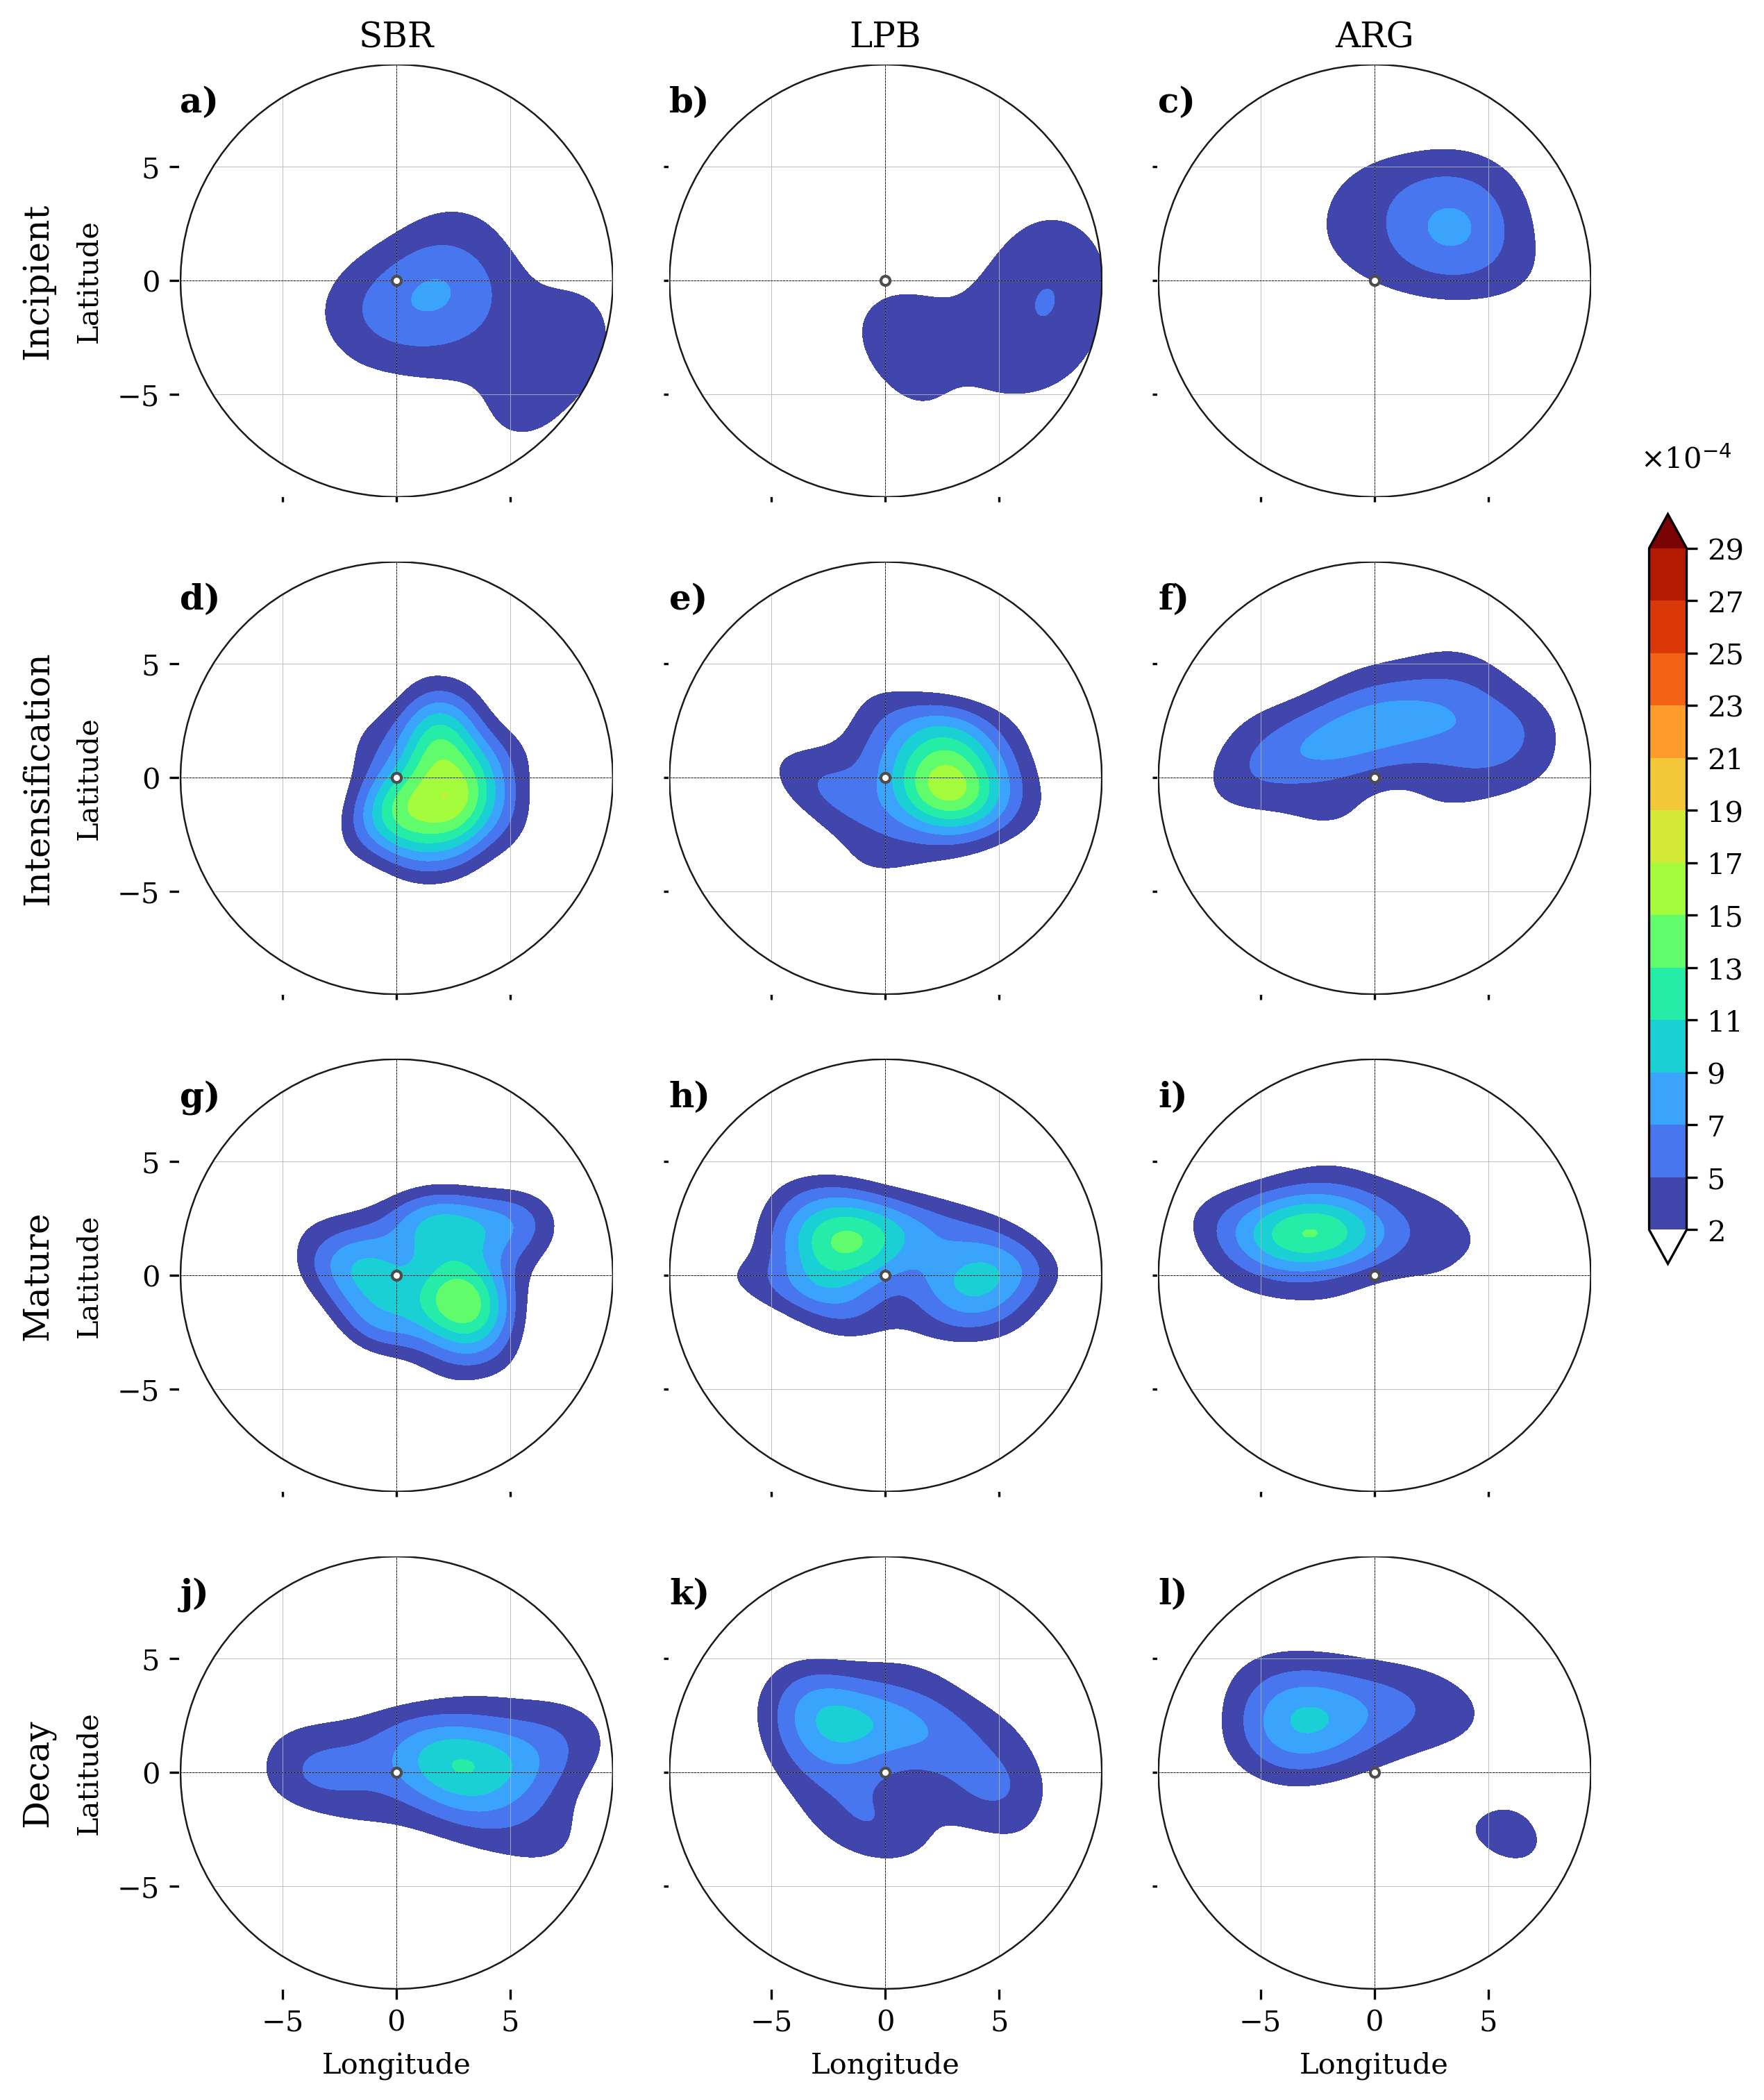
\includegraphics[width=\textwidth]{images/w100/kde_wind100_p50_fasesxreg.png}
% \caption[KDE espacial de viento a 100 m - Subconjunto p50]{Estimación de densidad espacial bidimensional (KDE) para la ubicación de los máximos de magnitud de viento a 100 metros en el estrato de ciclones moderados (percentil 50). El mapa evidencia un grado de organización cinemática intermedio: los núcleos de máxima probabilidad logran agruparse débilmente en los cuadrantes occidentales durante la madurez, delineando la influencia del sector frío, pero sin alcanzar jamás la hiperconcentración destructiva y focalizada propia de los eventos severos (p90).}
% \label{fig:kde_wind100_p50_ap}
% \end{figure}


\section{Precipitación total}\label{apendice:kde_tp}

\subsection{Sistemas débiles (p10)}\label{apendice:kde_tp_p10}
\begin{figure}[htbp]
\centering
\includegraphics[width=\textwidth]{images/tp/kde_tp_p10_fasesxreg.png}
\caption[KDE espacial de precipitación máxima - Subconjunto p10]{Estimación de densidad espacial bidimensional (KDE) para la ubicación de los máximos de precipitación total en el estrato de ciclones débiles (percentil 10). La topología marcadamente dispersa a lo largo de todo el ciclo de vida evidencia que los vórtices con forzante dinámico pobre no logran organizar bandas de precipitación coherentes, resultando en campos de lluvia espacialmente aleatorios.}
\label{fig:kde_tp_p10_ap}
\end{figure}

\subsection{Sistemas moderados (p50)}\label{apendice:kde_tp_p50}
\begin{figure}[htbp]
\centering
\includegraphics[width=\textwidth]{images/tp/kde_tp_p50_fasesxreg.png}
\caption[KDE espacial de precipitación máxima - Subconjunto p50]{Estimación de densidad espacial bidimensional (KDE) para la ubicación de los máximos de precipitación total en el estrato de ciclones típicos o moderados (percentil 50). El mapa refleja una concentración temprana y acentuada en el cuadrante sureste durante la intensificación, muy similar al comportamiento promediado de la Población Global, antes de sucumbir a la dispersión periférica típica de la oclusión en la madurez.}
\label{fig:kde_tp_p50_ap}
\end{figure}


% ==============================================================================
% EOF - APÉNDICE
% ==============================================================================
\chapter{Patrones espaciales adicionales (EOF)}\label{apendice:eof}

En este apéndice se documentan los primeros modos espaciales (EOF1) correspondientes a los estratos de menor intensidad dinámica (p10 y p50), complementando los análisis principales del texto. Estos mapas demuestran cómo la estructura espacial de la varianza depende inherentemente del potencial de profundización del sistema.

\section{Viento a 10 metros}\label{apendice:eof_wind10}

\subsection{Sistemas débiles (p10)}\label{apendice:eof1_wind10_p10}
\begin{figure}[htbp]
\centering
\includegraphics[width=\textwidth]{images/w10/pca1_wind10_p10_fasesxreg.png}
\caption[EOF1 de viento a 10 m - Subconjunto p10]{Primer modo espacial (EOF1) de la magnitud del viento a 10 metros para el subconjunto de ciclones débiles (percentil 10). La varianza explicada fluctúa entre $28.4\%$ y $36.5\%$. El patrón retiene un dipolo de fondo sumamente desorganizado, reflejando sistemas donde la falta de profundización dinámica impide la consolidación de un campo de viento con firmas estructurales coherentes.}
\label{fig:eof1_wind10_p10_ap}
\end{figure}

\subsection{Sistemas moderados (p50)}\label{apendice:eof1_wind10_p50}
\begin{figure}[htbp]
\centering
\includegraphics[width=\textwidth]{images/w10/pca1_wind10_p50_fasesxreg.png}
\caption[EOF1 de viento a 10 m - Subconjunto p50]{Primer modo espacial (EOF1) de la magnitud del viento a 10 metros para el subconjunto de ciclones típicos o moderados (percentil 50). La diferencia estructural frente al comportamiento climatológico comienza a ser evidente: la varianza explicada cae (con mínimos del $21.3\%$ en ARG) y el dipolo sufre distorsiones, mostrando características propias de sistemas que poseen mayor organización baroclínica pero sin alcanzar la severidad mesoescalar del grupo extremo.}
\label{fig:eof1_wind10_p50_ap}
\end{figure}

% \section{Viento a 100 metros}\label{apendice:eof_wind100}

% \subsection{Sistemas débiles (p10)}\label{apendice:eof1_wind100_p10}
% \begin{figure}[htbp]
% \centering
% \includegraphics[width=\textwidth]{images/w100/pca1_wind100_p10_fasesxreg.png}
% \caption[EOF1 de viento a 100 m - Subconjunto p10]{Primer modo espacial (EOF1) de la magnitud del viento a 100 metros para el estrato de ciclones débiles (percentil 10). La varianza explicada se sitúa entre el $26.1\%$ y el $41.0\%$. El patrón muestra una dispersión acentuada del dipolo de fondo, propia de sistemas que carecen del forzamiento termodinámico mínimo para organizar un campo de viento coherente.}
% \label{fig:eof1_wind100_p10_ap}
% \end{figure}

% \subsection{Sistemas moderados (p50)}\label{apendice:eof1_wind100_p50}
% \begin{figure}[htbp]
% \centering
% 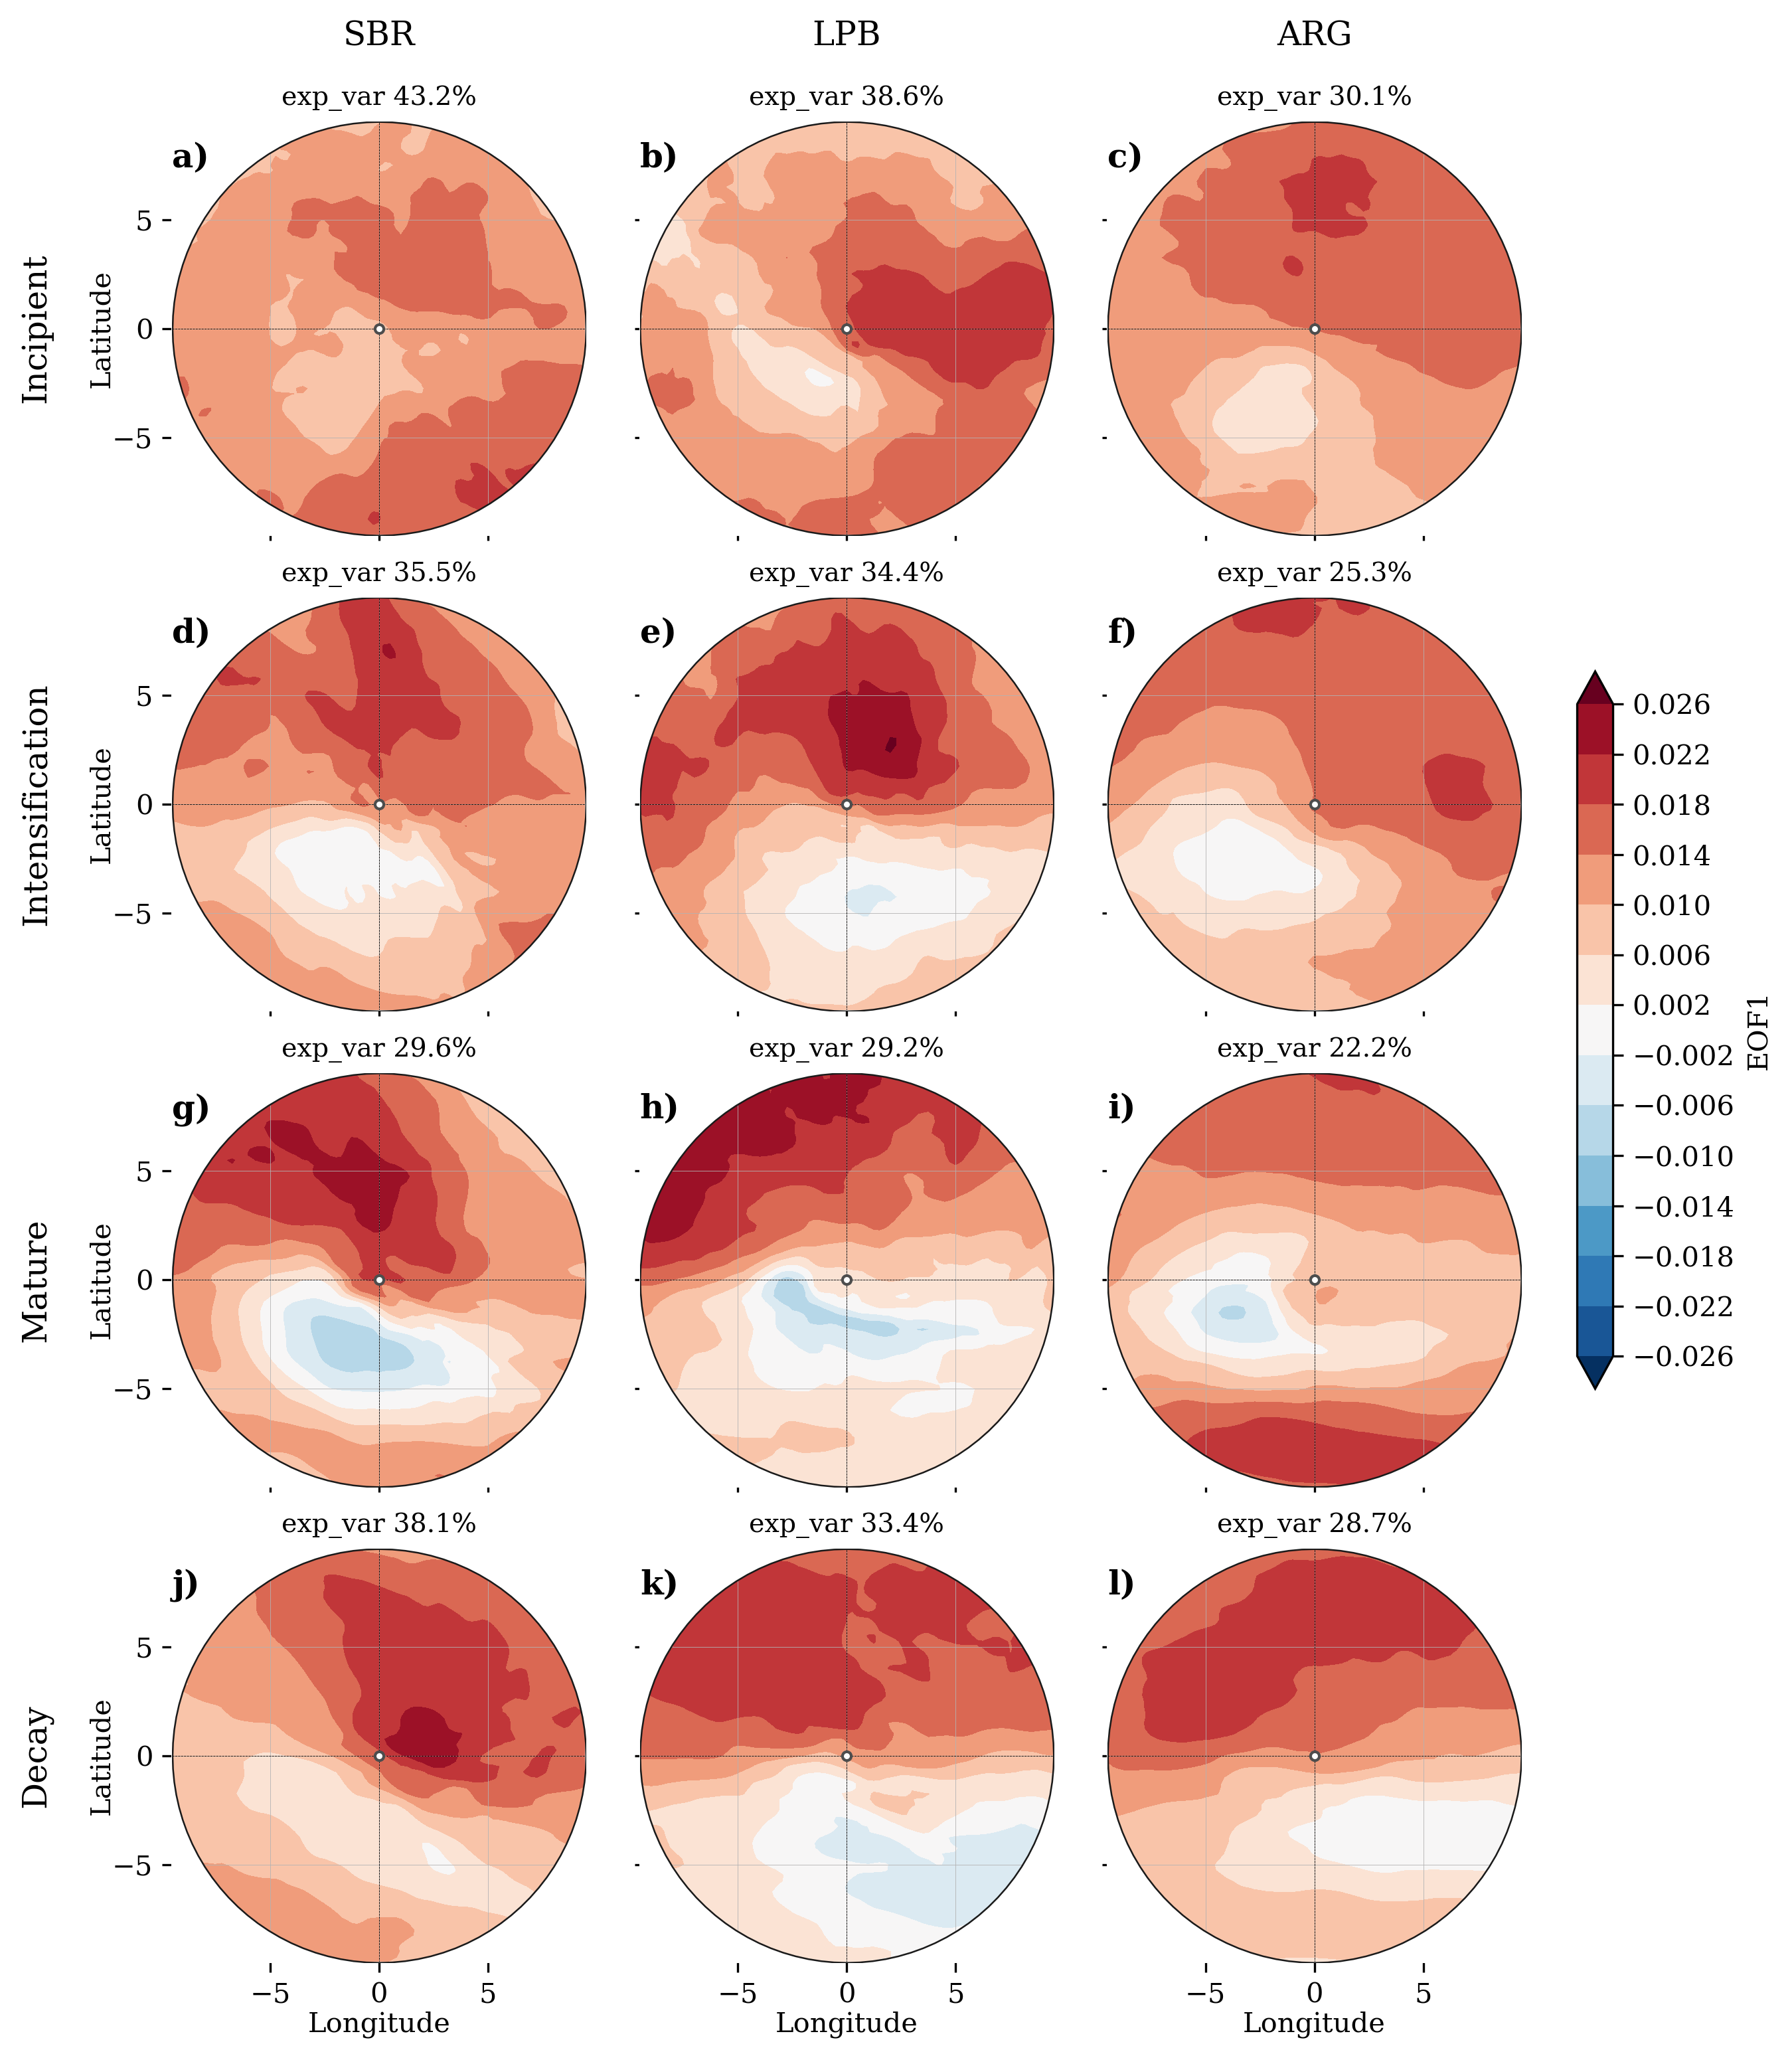
\includegraphics[width=\textwidth]{images/w100/pca1_wind100_p50_fasesxreg.png}
% \caption[EOF1 de viento a 100 m - Subconjunto p50]{Primer modo espacial (EOF1) de la magnitud del viento a 100 metros para el estrato de ciclones moderados (percentil 50). La varianza explicada oscila entre el $22.2\%$ y el $43.2\%$. El patrón representa el grado intermedio de organización estructural, donde el flujo de fondo comienza a verse distorsionado por la rotación interna del ciclón promedio, aunque sin alcanzar la hiperconcentración de los eventos severos.}
% \label{fig:eof1_wind100_p50_ap}
% \end{figure}

%

\section{Precipitación total (EOF)}\label{apendice:eof_tp}

\subsection{Sistemas débiles (p10)}\label{apendice:eof1_tp_p10}
\begin{figure}[htbp]
\centering
\includegraphics[width=\textwidth]{images/tp/pca1_tp_p10_fasesxreg.png}
\caption[EOF1 de precipitación total - Subconjunto p10]{Primer modo espacial (EOF1) de la precipitación total para el estrato de ciclones débiles (percentil 10). La varianza explicada oscila entre el $9.2\%$ y el $17.2\%$. El patrón retiene la banda sureste pero de forma fragmentada y amorfa, confirmando que la carencia de forzamiento dinámico profundo impide la organización estructural de la convección a gran escala.}
\label{fig:eof1_tp_p10_ap}
\end{figure}

\subsection{Sistemas moderados (p50)}\label{apendice:eof1_tp_p50}
\begin{figure}[htbp]
\centering
\includegraphics[width=\textwidth]{images/tp/pca1_tp_p50_fasesxreg.png}
\caption[EOF1 de precipitación total - Subconjunto p50]{Primer modo espacial (EOF1) de la precipitación total para el estrato de ciclones moderados (percentil 50). La varianza explicada se consolida entre el $9.7\%$ y el $18.4\%$. Este estrato refleja una banda frontal sureste mucho más definida que el p10, operando como el paso intermedio de organización estructural antes del severo enroscamiento (\textit{wrap-around}) que caracteriza a los eventos extremos del p90.}
\label{fig:eof1_tp_p50_ap}
\end{figure}
%%%%%%%%%%%%%%
% ==============================================================================
% ==============================================================================
% ==============================================================================
% XEOF MULTIDIMENSIONAL - APÉNDICE
% ==============================================================================

\chapter{Análisis Multidimensional del Viento a 10 metros: Fases Evolutivas Adicionales}\label{apendice:xeof_fases}

Este apéndice complementa el análisis multidimensional presentado en la sección de resultados. A continuación, se documentan los patrones espaciales (EOF1, EOF2, EOF3) con sus respectivas zonas de significancia estadística (calculadas mediante \textit{bootstrapping} con 15,000 iteraciones) y las PCs para las etapas incipiente, de intensificación y decaimiento.

Se contrastan los resultados de la Población Global de referencia (climatología general) frente al subconjunto de eventos dinámicamente extremos (percentil 90), permitiendo observar la evolución temporal completa de las asimetrías estructurales.

% ------------------------------------------------------------------------------
\section{Población Global}
% ------------------------------------------------------------------------------

\begin{figure}[htbp]
\centering
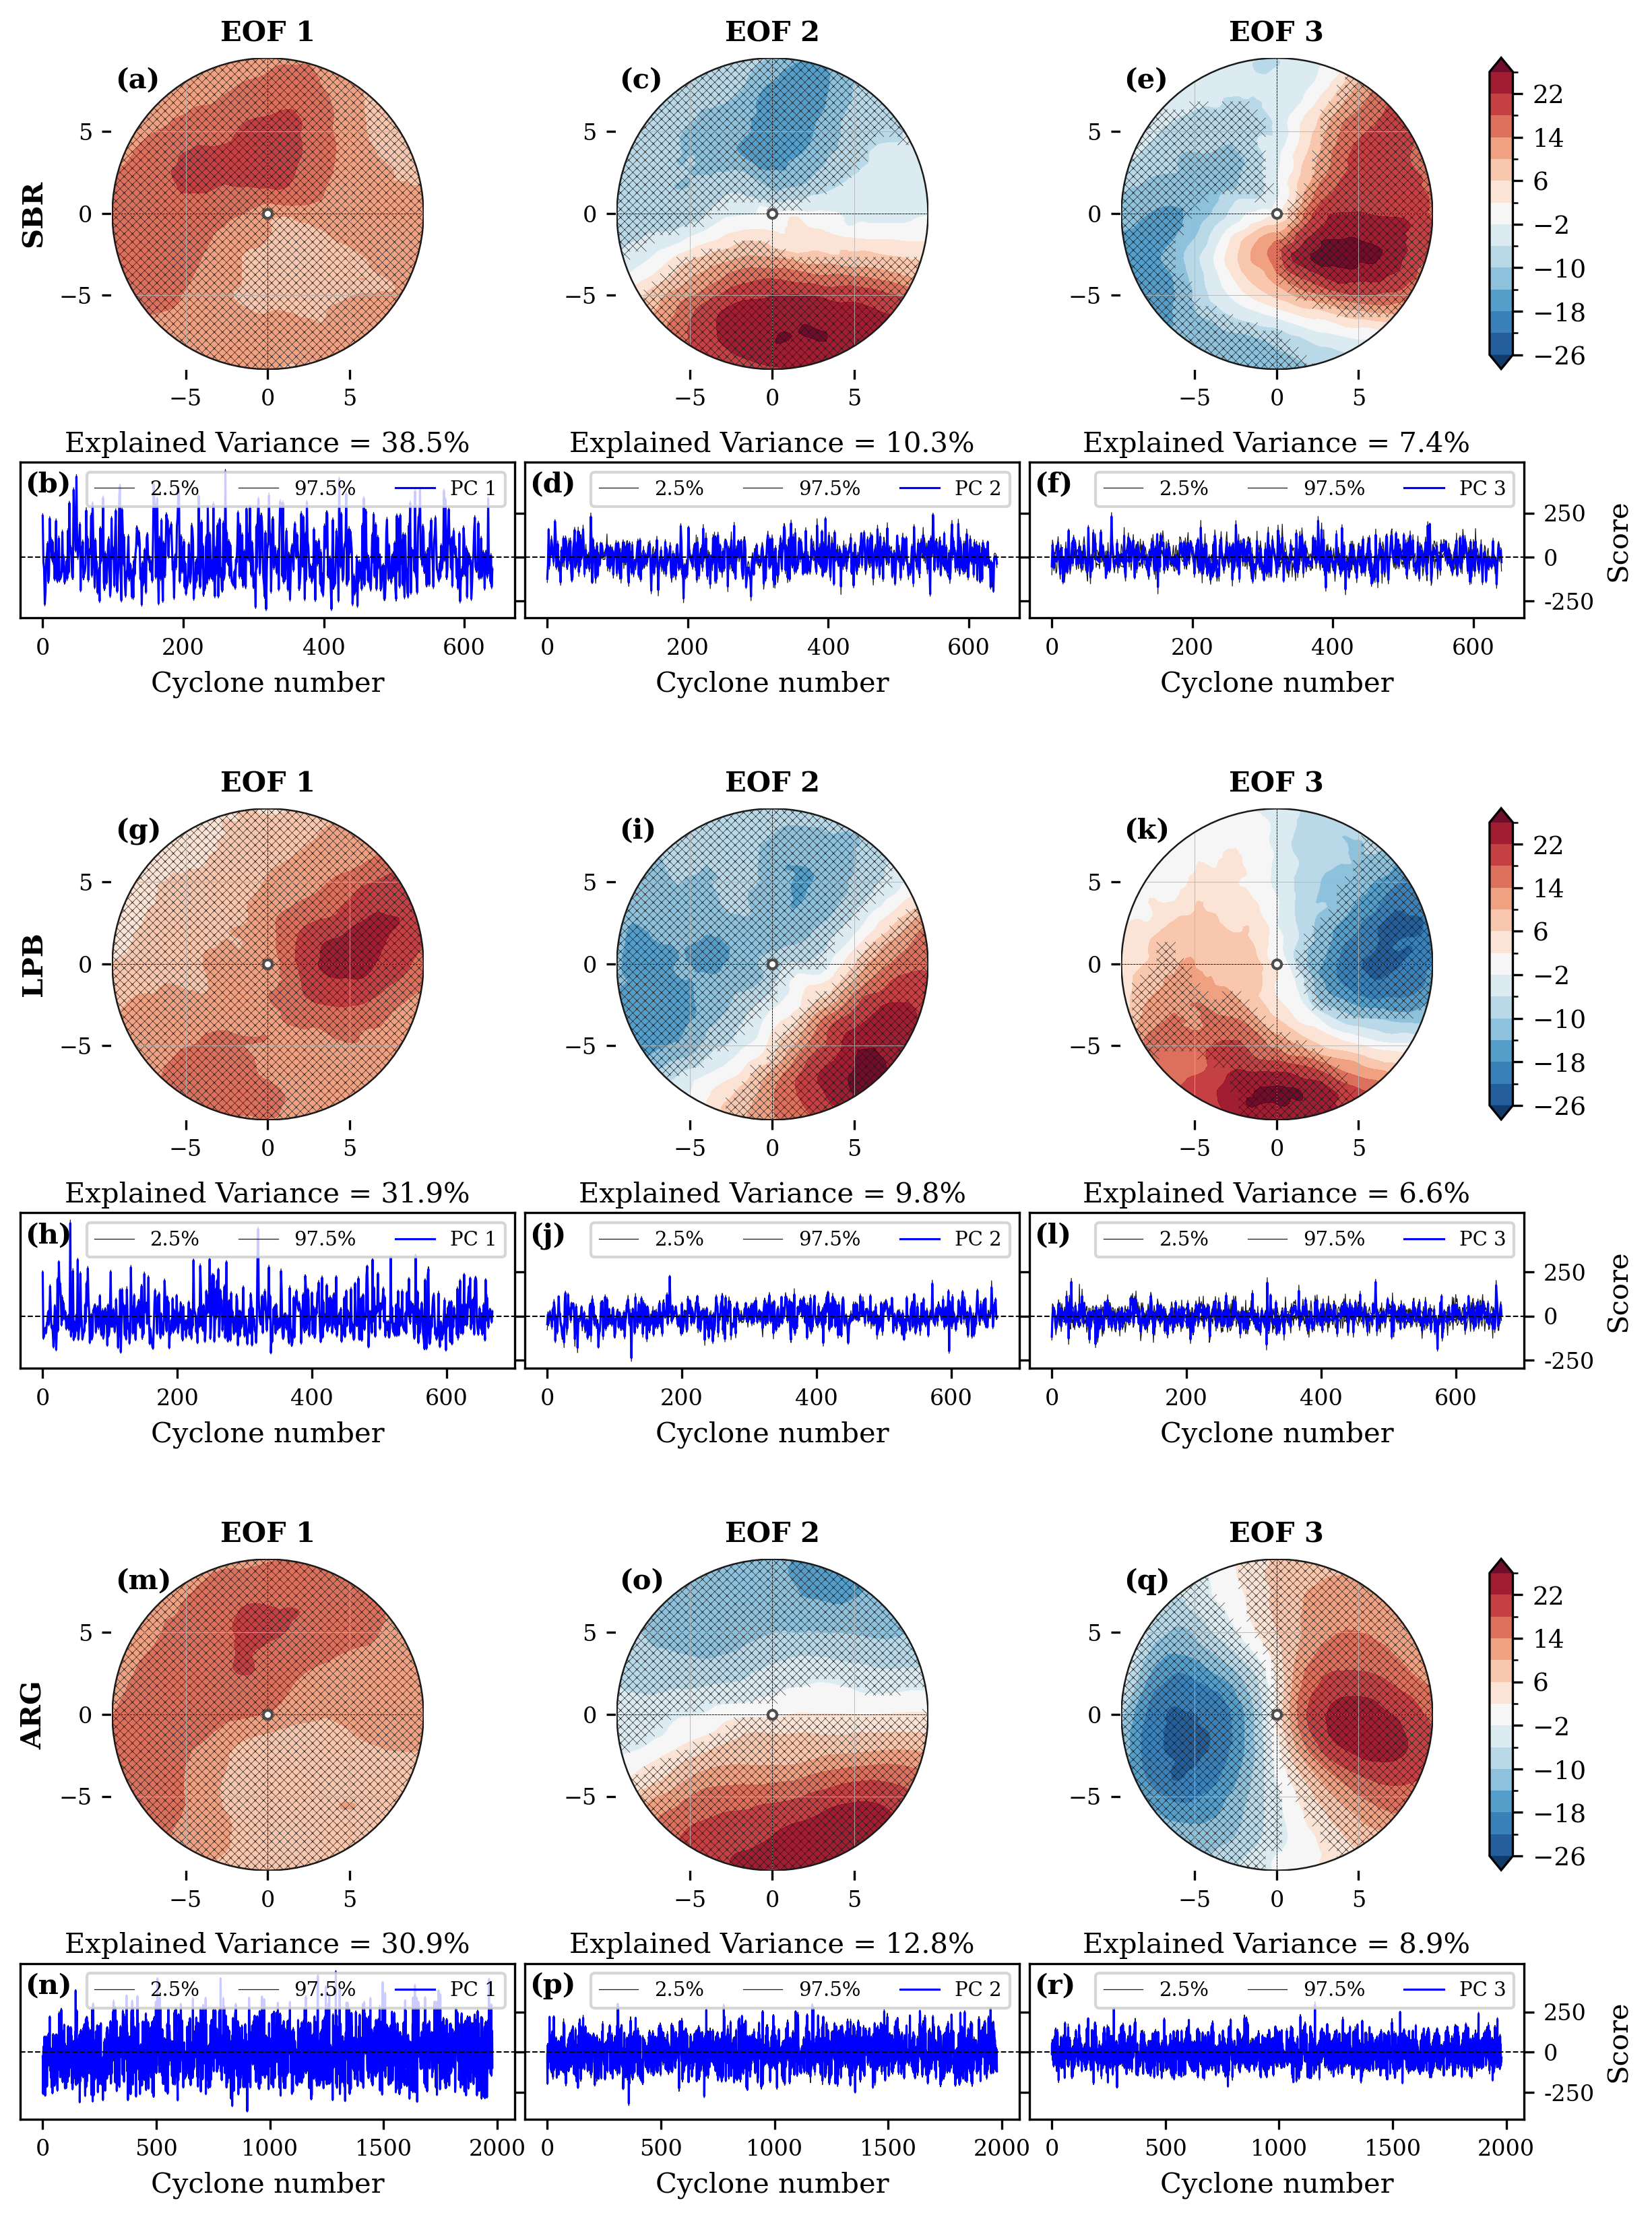
\includegraphics[width=\textwidth]{images/w10/xeof_global_wind10_incipient.jpg}
\caption[EOF1-3  - Población Global (Incipiente)]{Análisis multidimensional del viento a 10 metros para la \textbf{Población Global} durante la \textbf{fase incipiente}. Las zonas punteadas indican significancia estadística al 95\% empírico.}
\label{fig:apendice_global_incipiente}
\end{figure}

\begin{figure}[htbp]
\centering
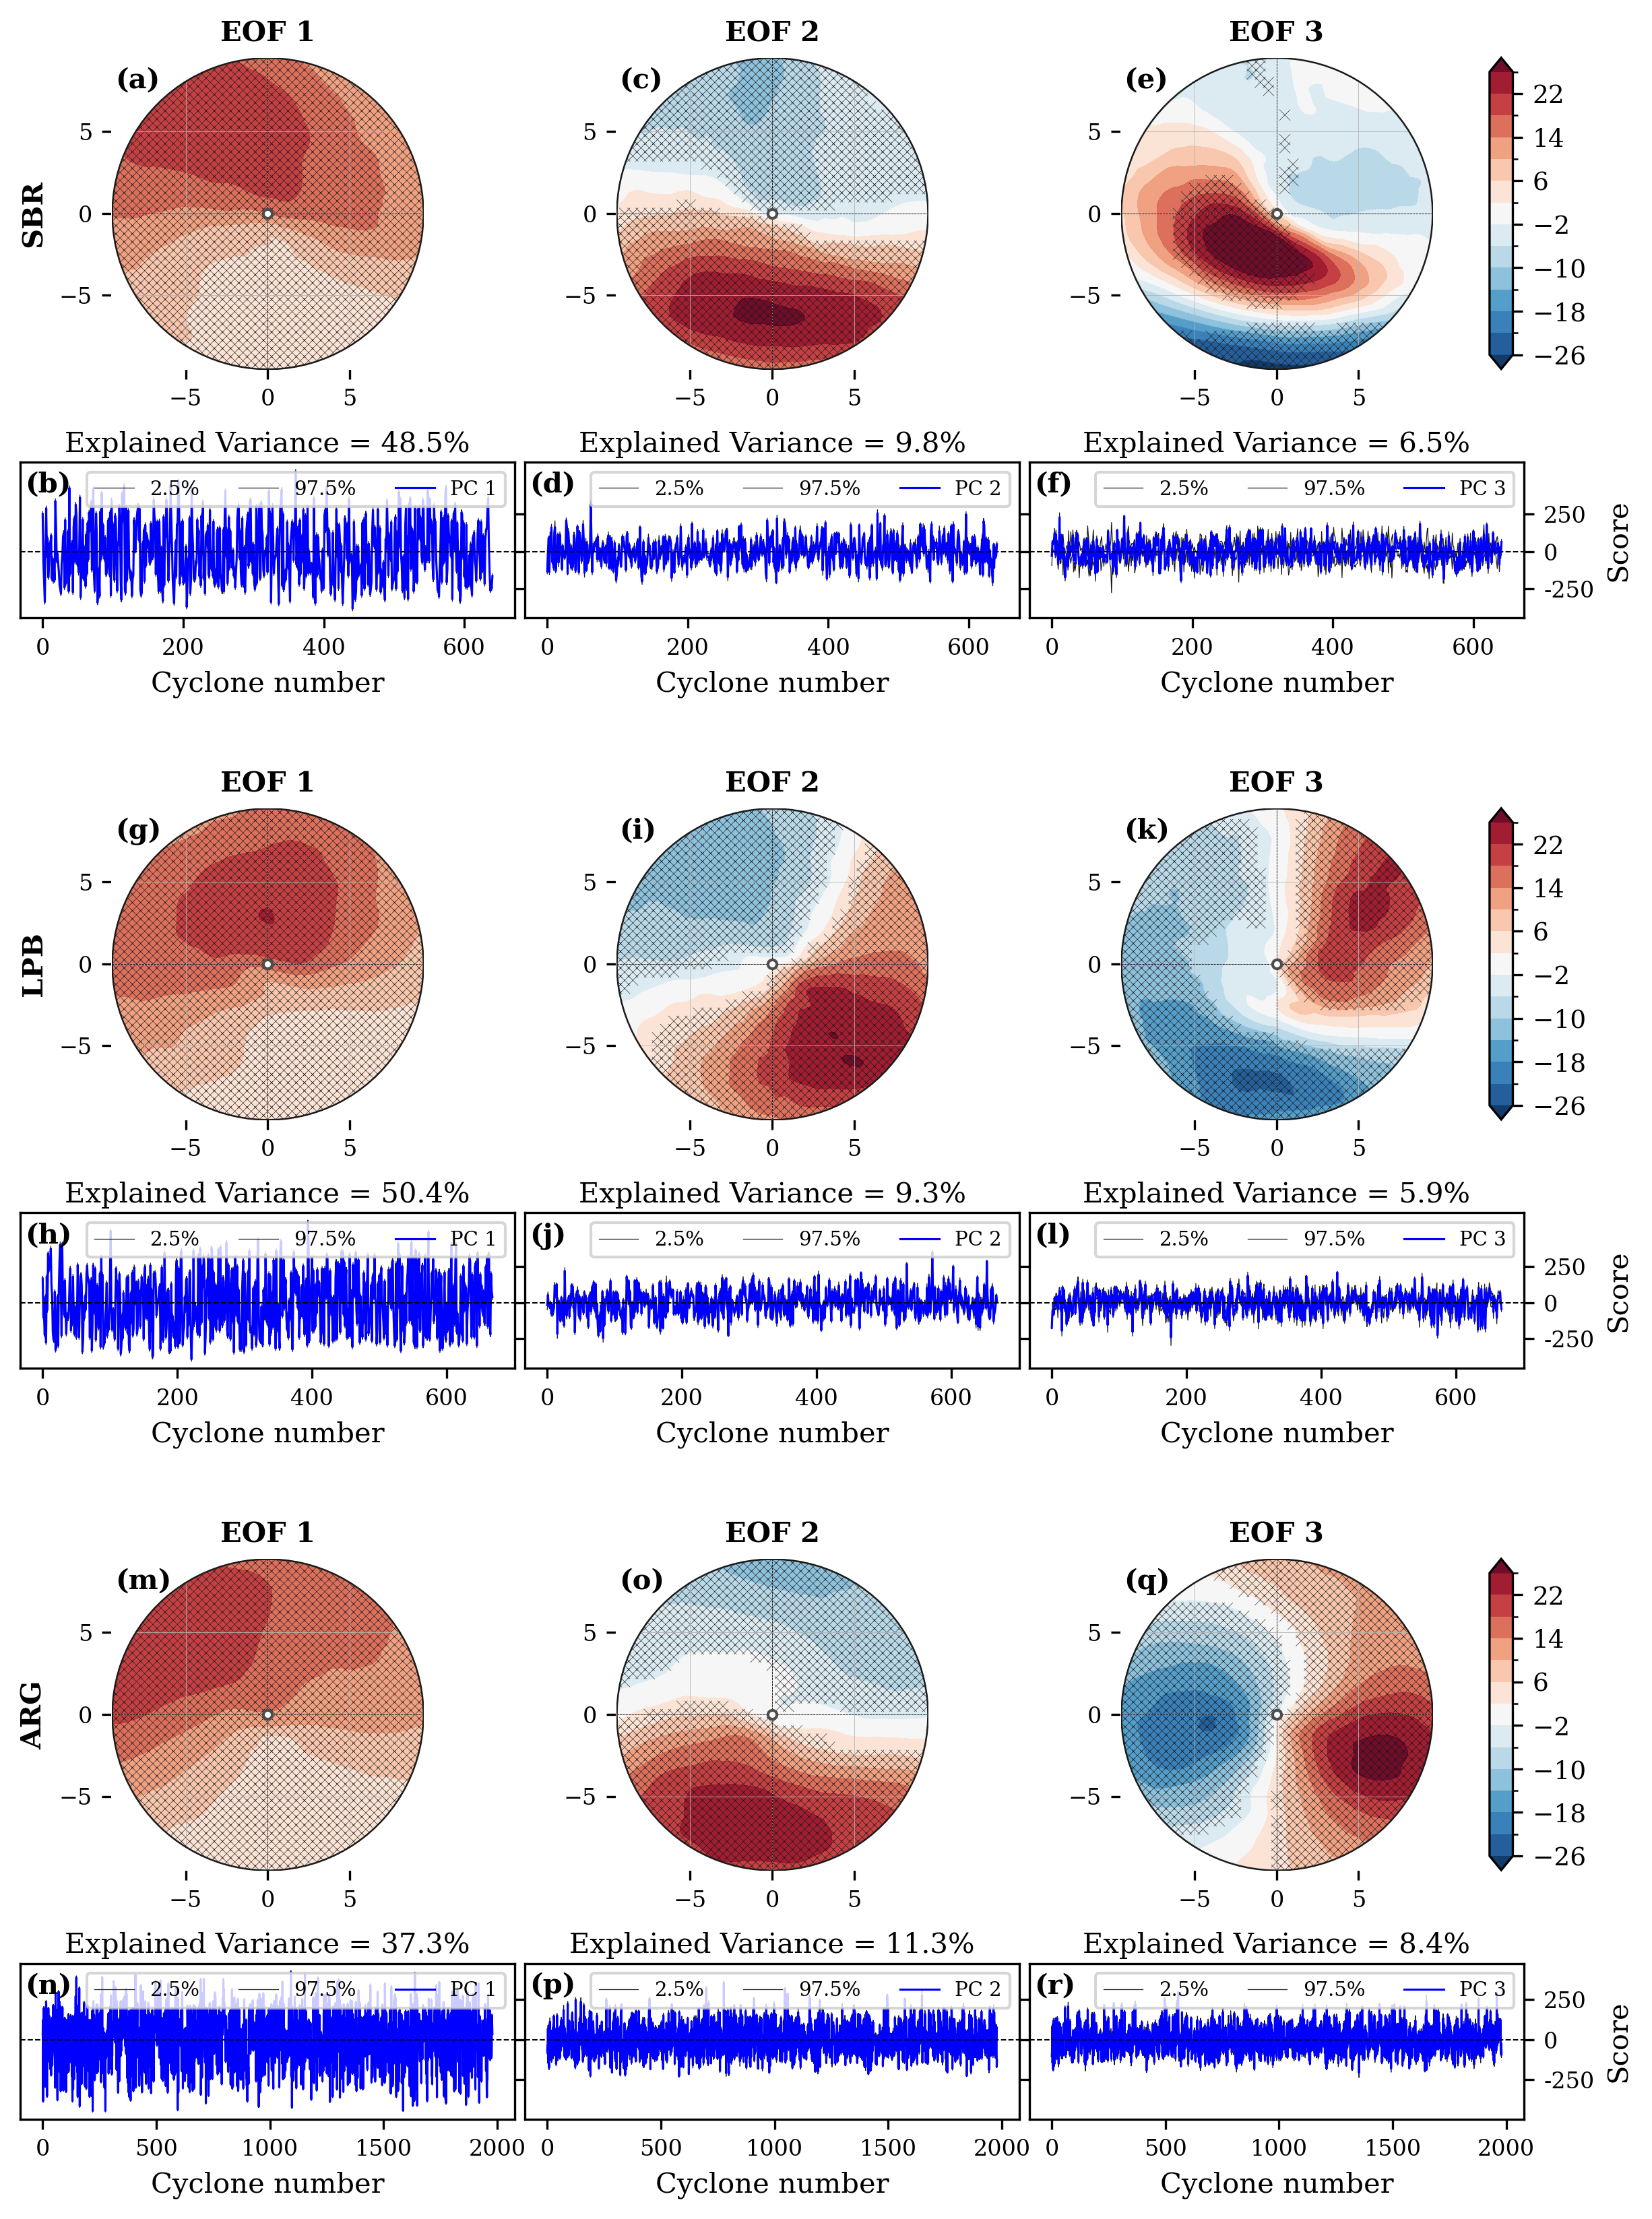
\includegraphics[width=\textwidth]{images/w10/xeof_global_wind10_intensification.jpg}
\caption[EOF1-3  - Población Global (Intensificación)]{Análisis multidimensional del viento a 10 metros para la \textbf{Población Global} durante la \textbf{fase de intensificación}. Las zonas punteadas indican significancia estadística al 95\% empírico.}
\label{fig:apendice_global_intensificacion}
\end{figure}

\begin{figure}[htbp]
\centering
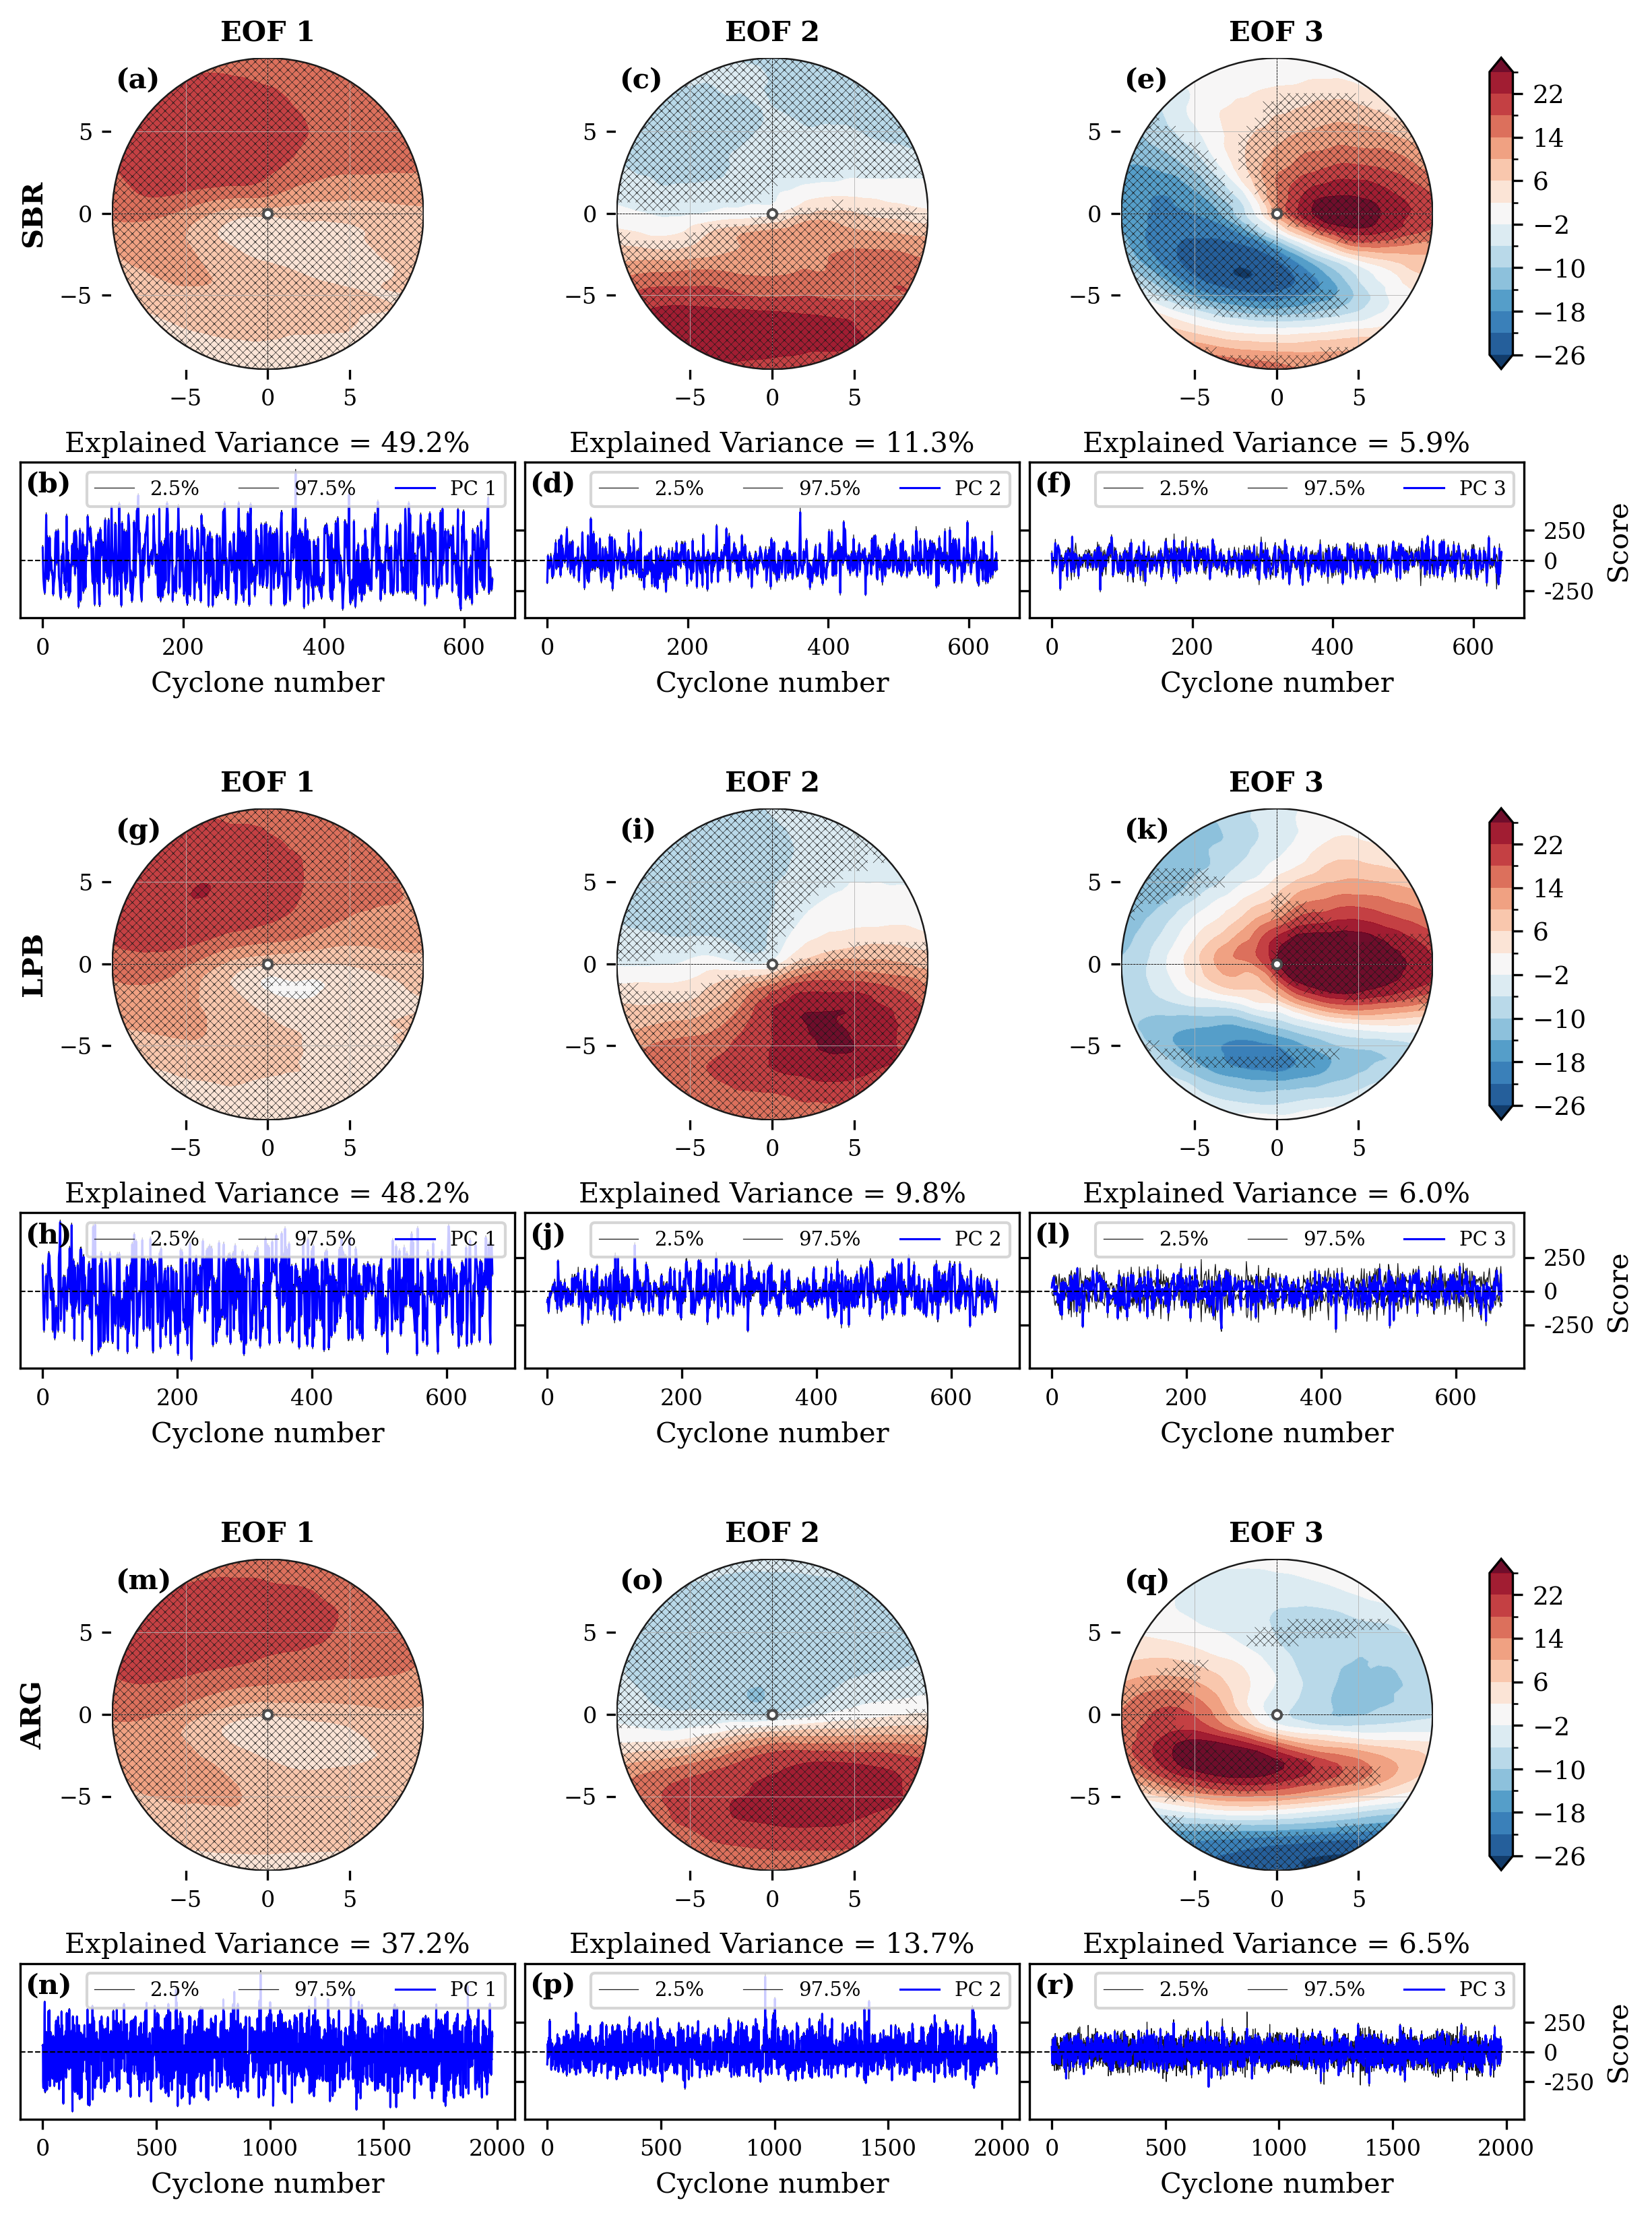
\includegraphics[width=\textwidth]{images/w10/xeof_global_wind10_decay.jpg}
\caption[EOF1-3  - Población Global (Decaimiento)]{Análisis multidimensional del viento a 10 metros para la \textbf{Población Global} durante la \textbf{fase de decaimiento}. Las zonas punteadas indican significancia estadística al 95\% empírico.}
\label{fig:apendice_global_decaimiento}
\end{figure}

\clearpage

% ------------------------------------------------------------------------------
\section{Subconjunto Extremo (p90)}
% ------------------------------------------------------------------------------

\begin{figure}[htbp]
\centering
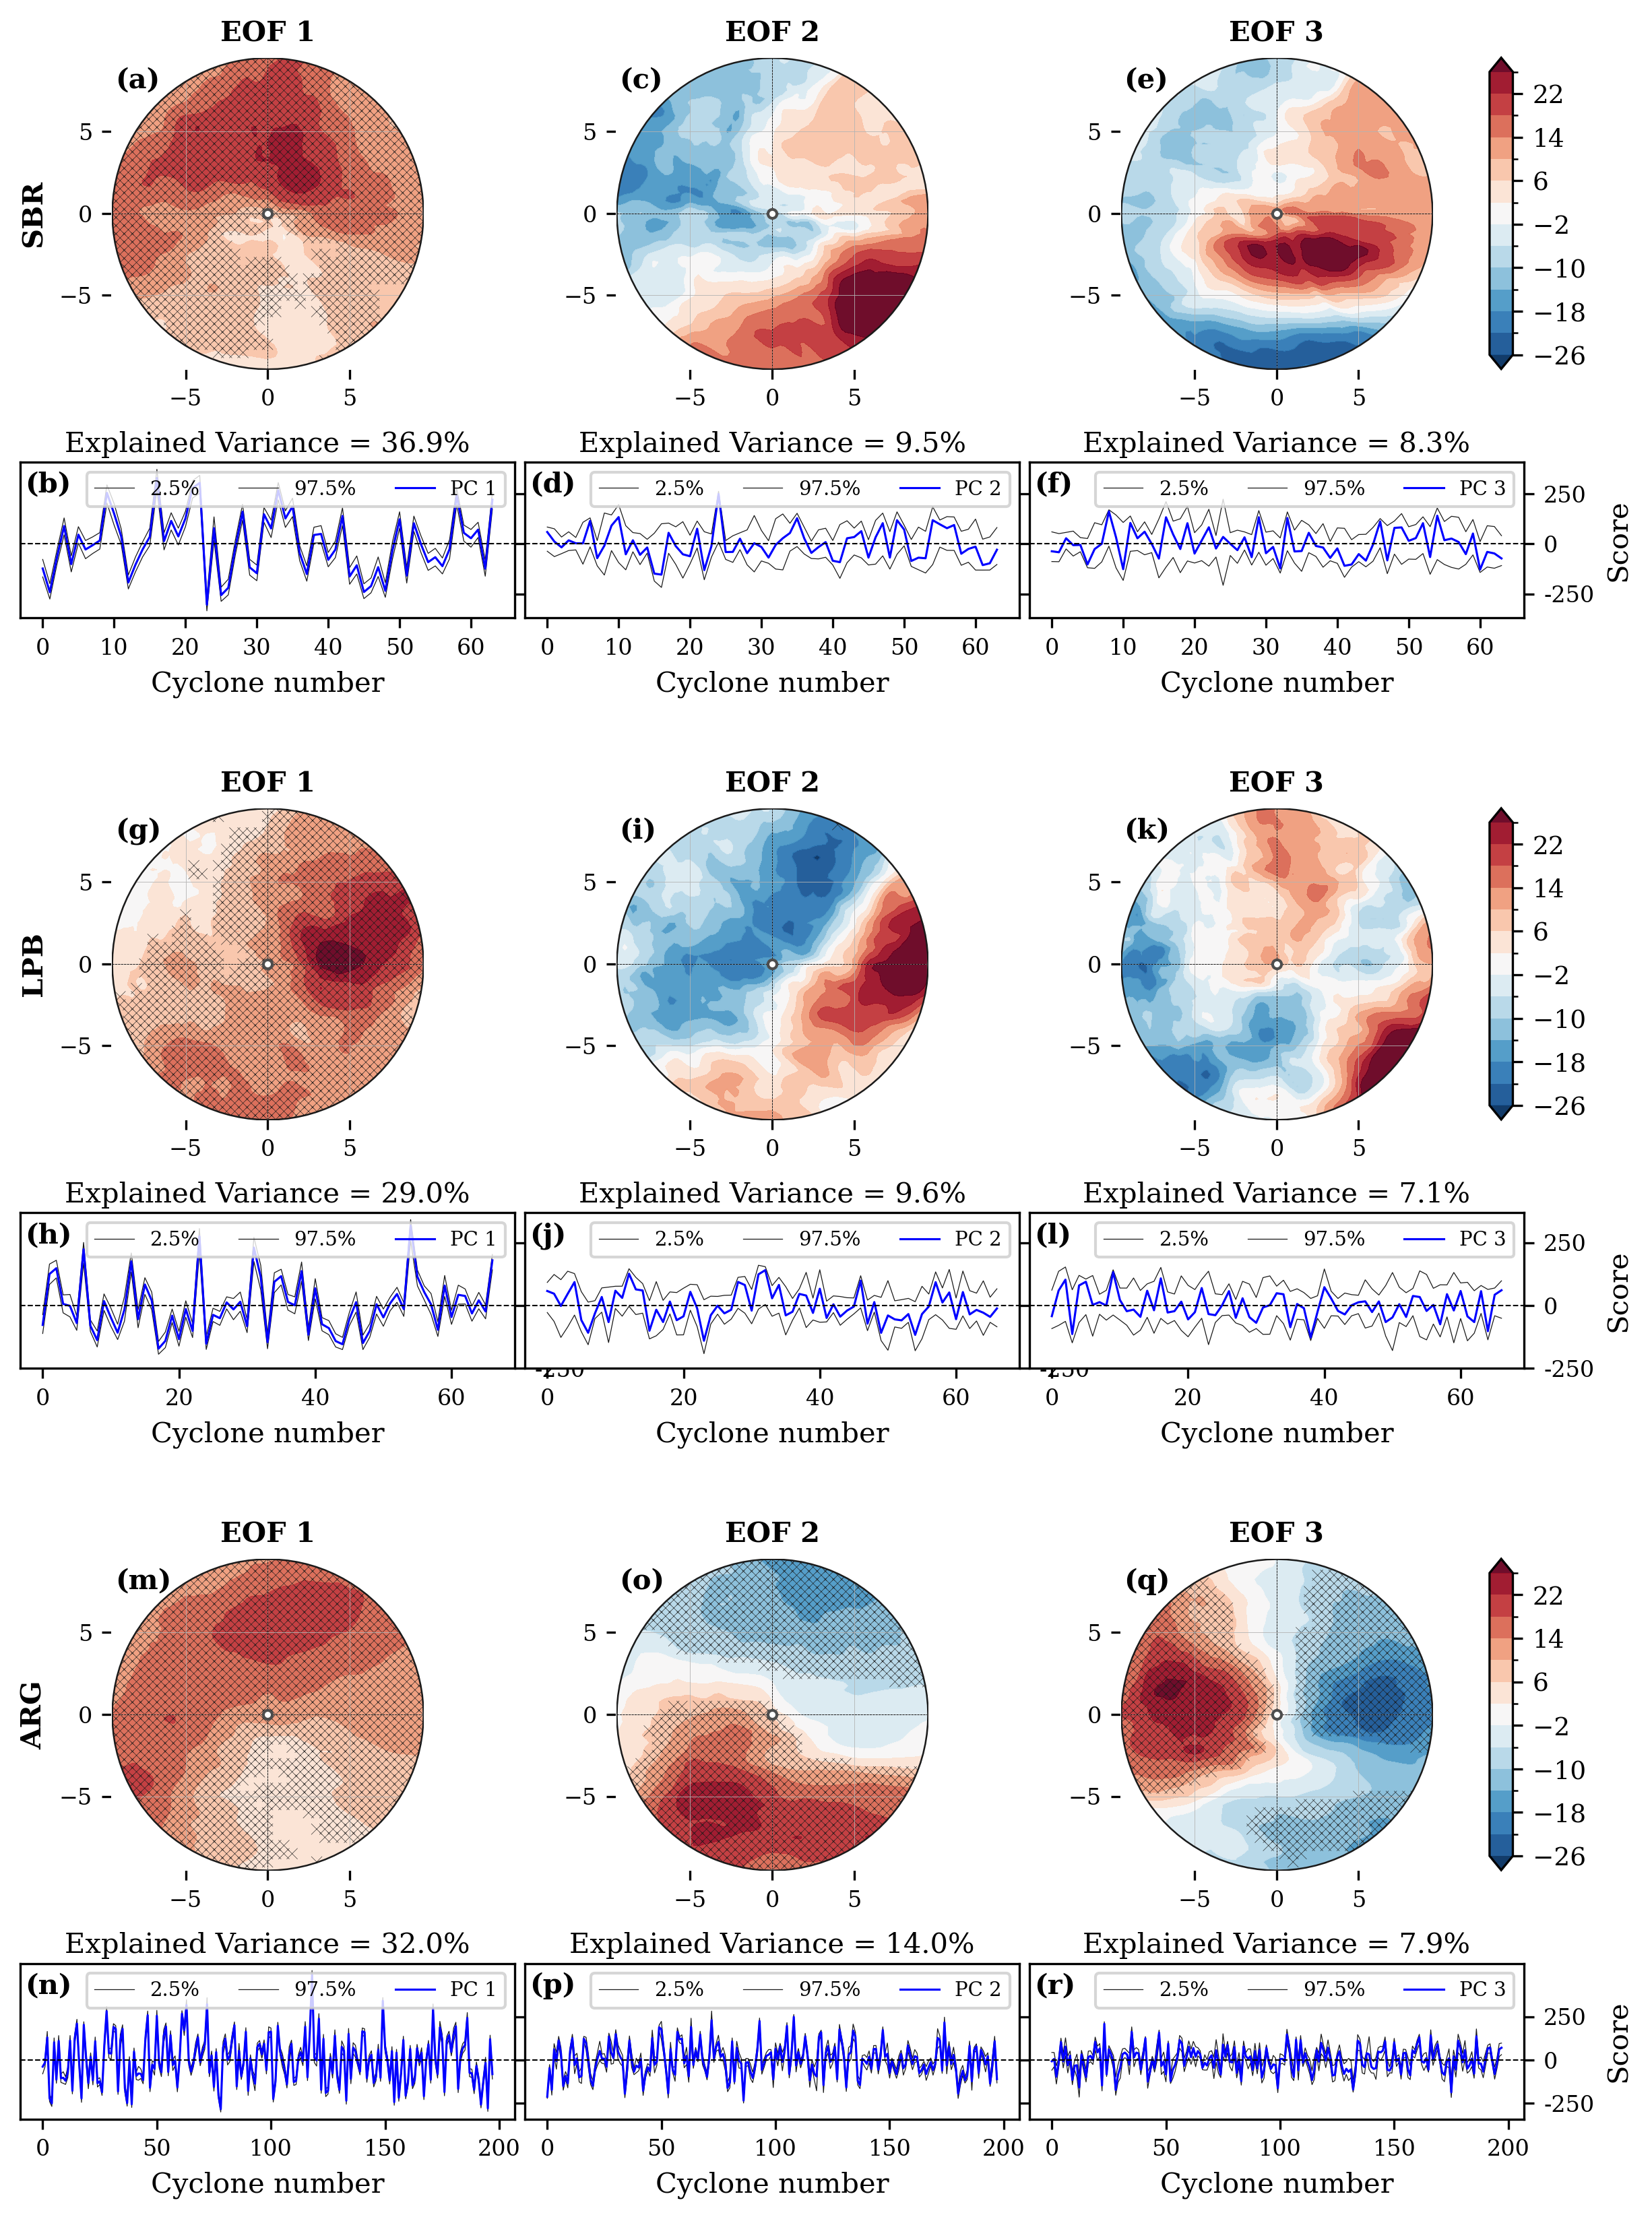
\includegraphics[width=\textwidth]{images/w10/xeof_p90_wind10_incipient.jpg}
\caption[EOF1-3  - Subconjunto p90 (Incipiente)]{Análisis multidimensional del viento a 10 metros para el \textbf{subconjunto extremo (p90)} durante la \textbf{fase incipiente}. Las zonas punteadas indican significancia estadística al 95\% empírico, evidenciando alteraciones tempranas respecto a la población global.}
\label{fig:apendice_p90_incipiente}
\end{figure}

\begin{figure}[htbp]
\centering
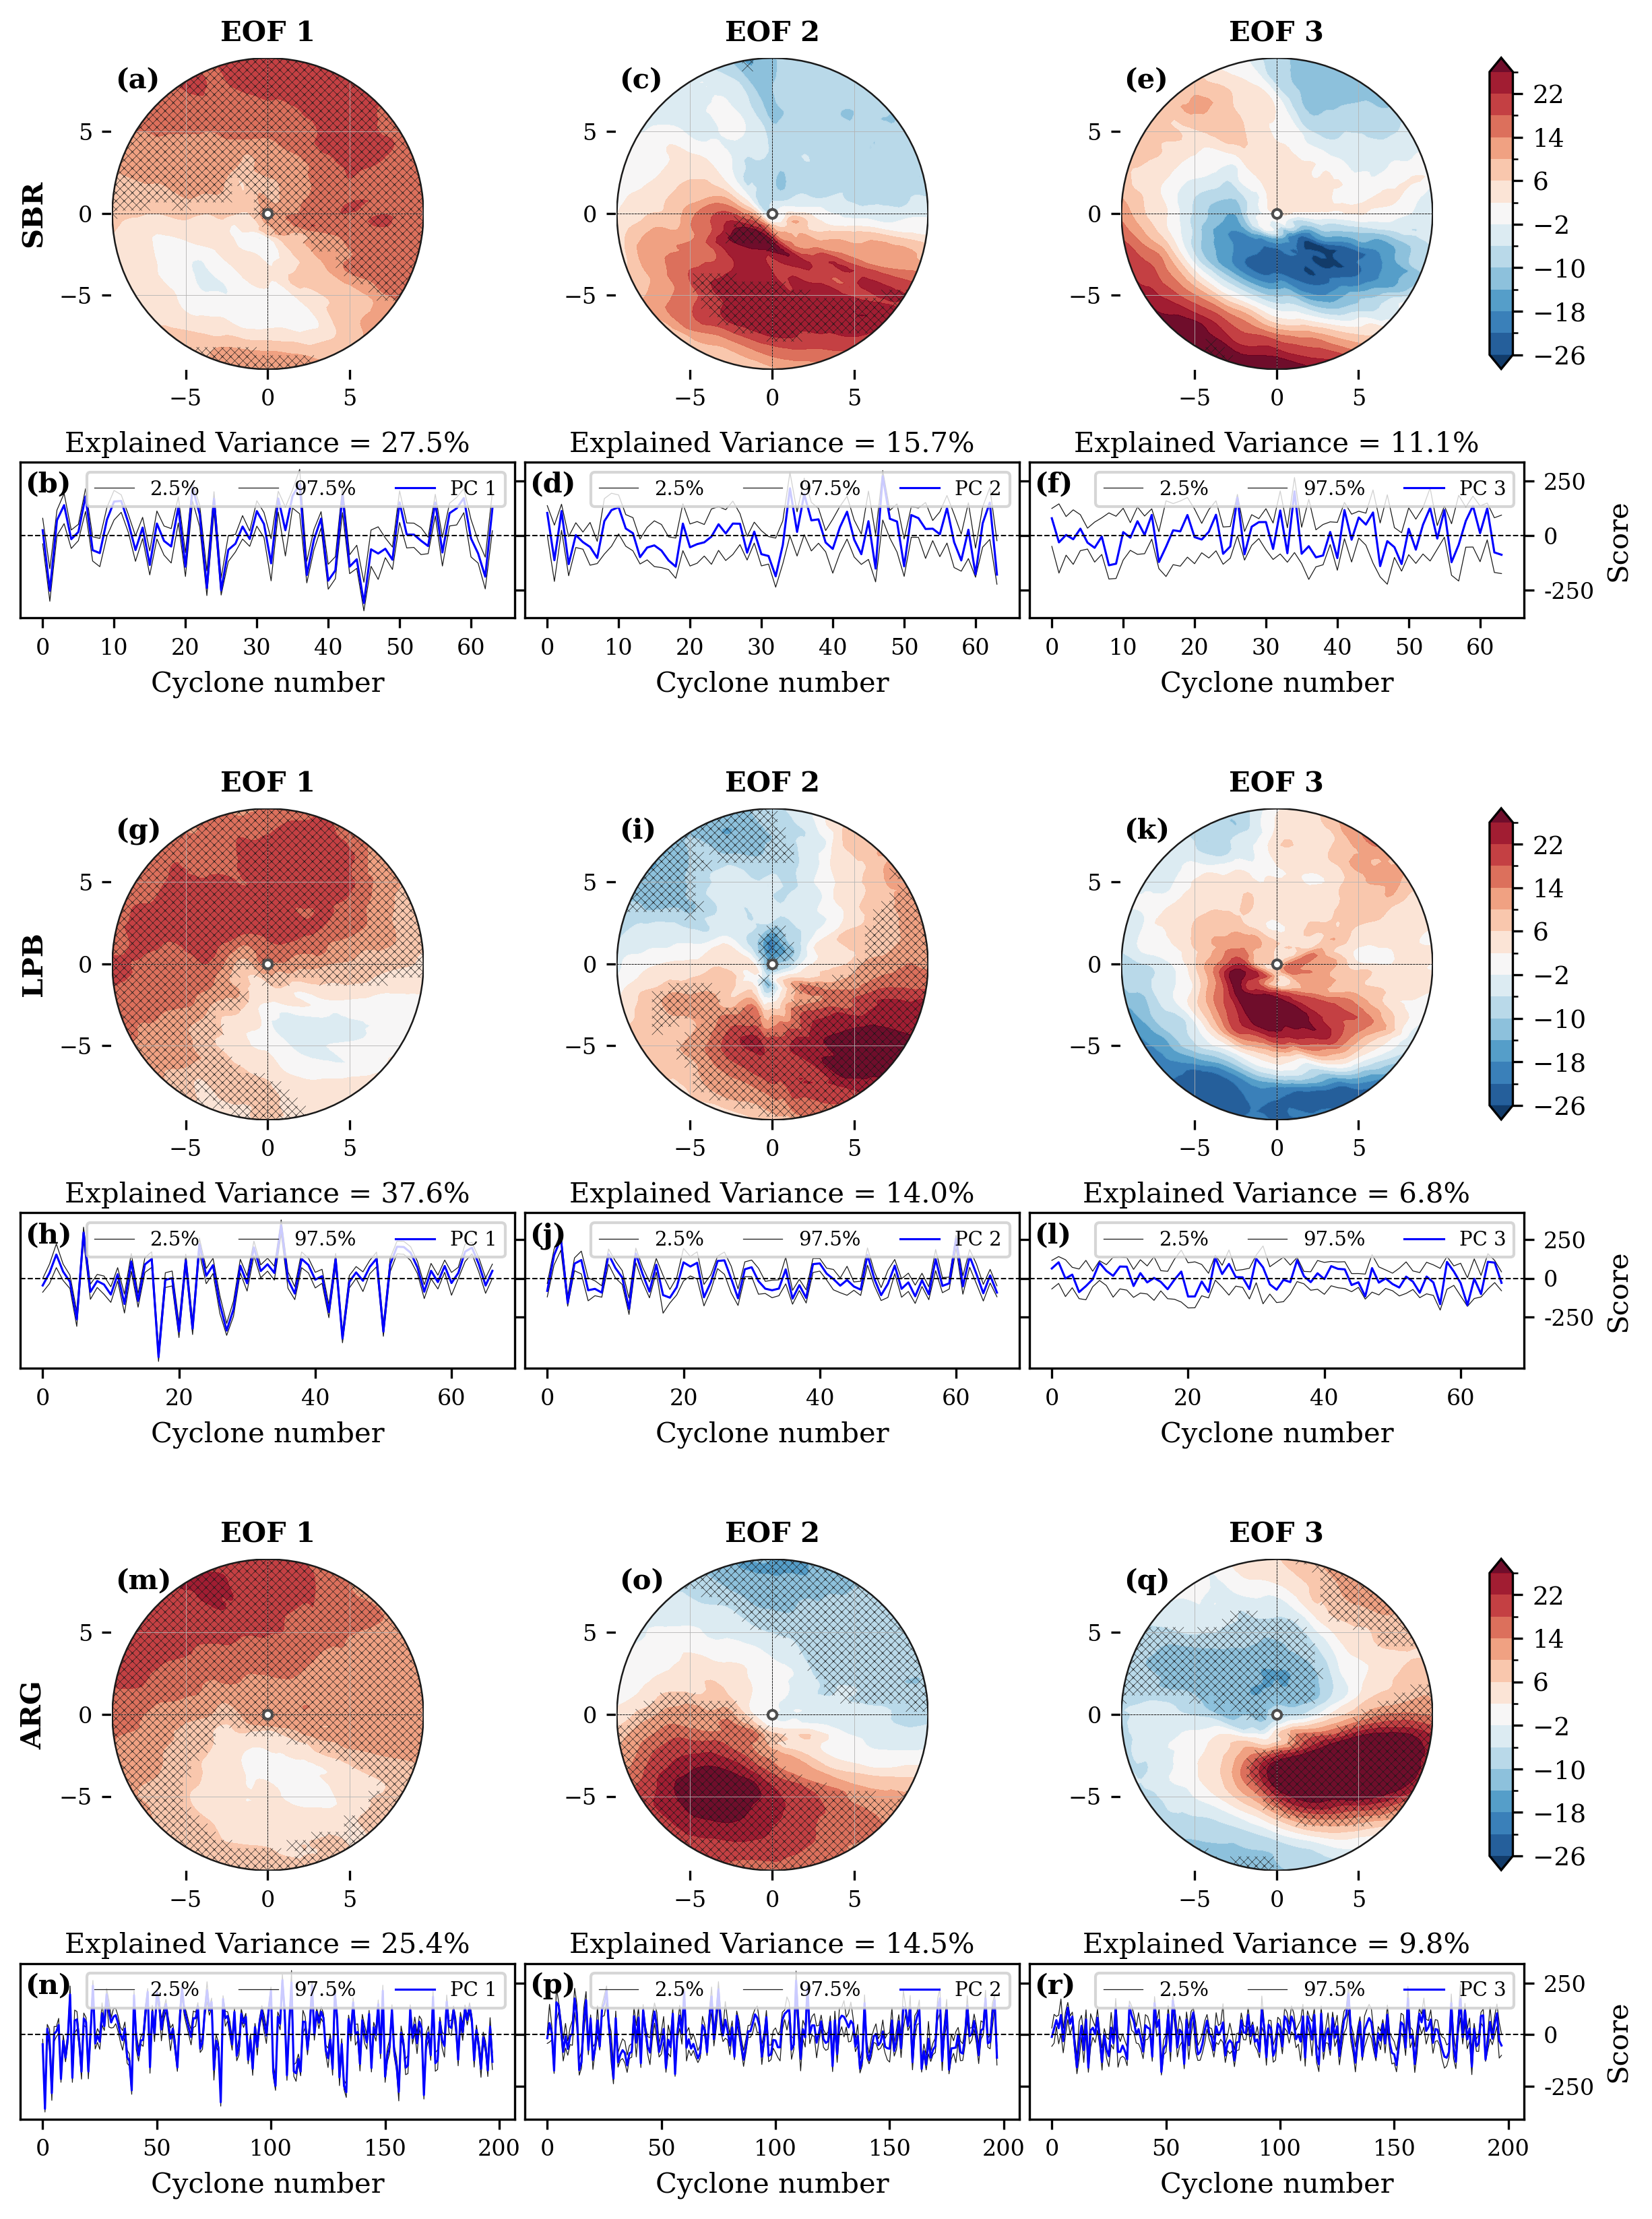
\includegraphics[width=\textwidth]{images/w10/xeof_p90_wind10_intensification.jpg}
\caption[EOF1-3  - Subconjunto p90 (Intensificación)]{Análisis multidimensional del viento a 10 metros para el \textbf{subconjunto extremo (p90)} durante la \textbf{fase de intensificación}. Las zonas punteadas indican significancia estadística al 95\% empírico.}
\label{fig:apendice_p90_intensificacion}
\end{figure}

\begin{figure}[htbp]
\centering
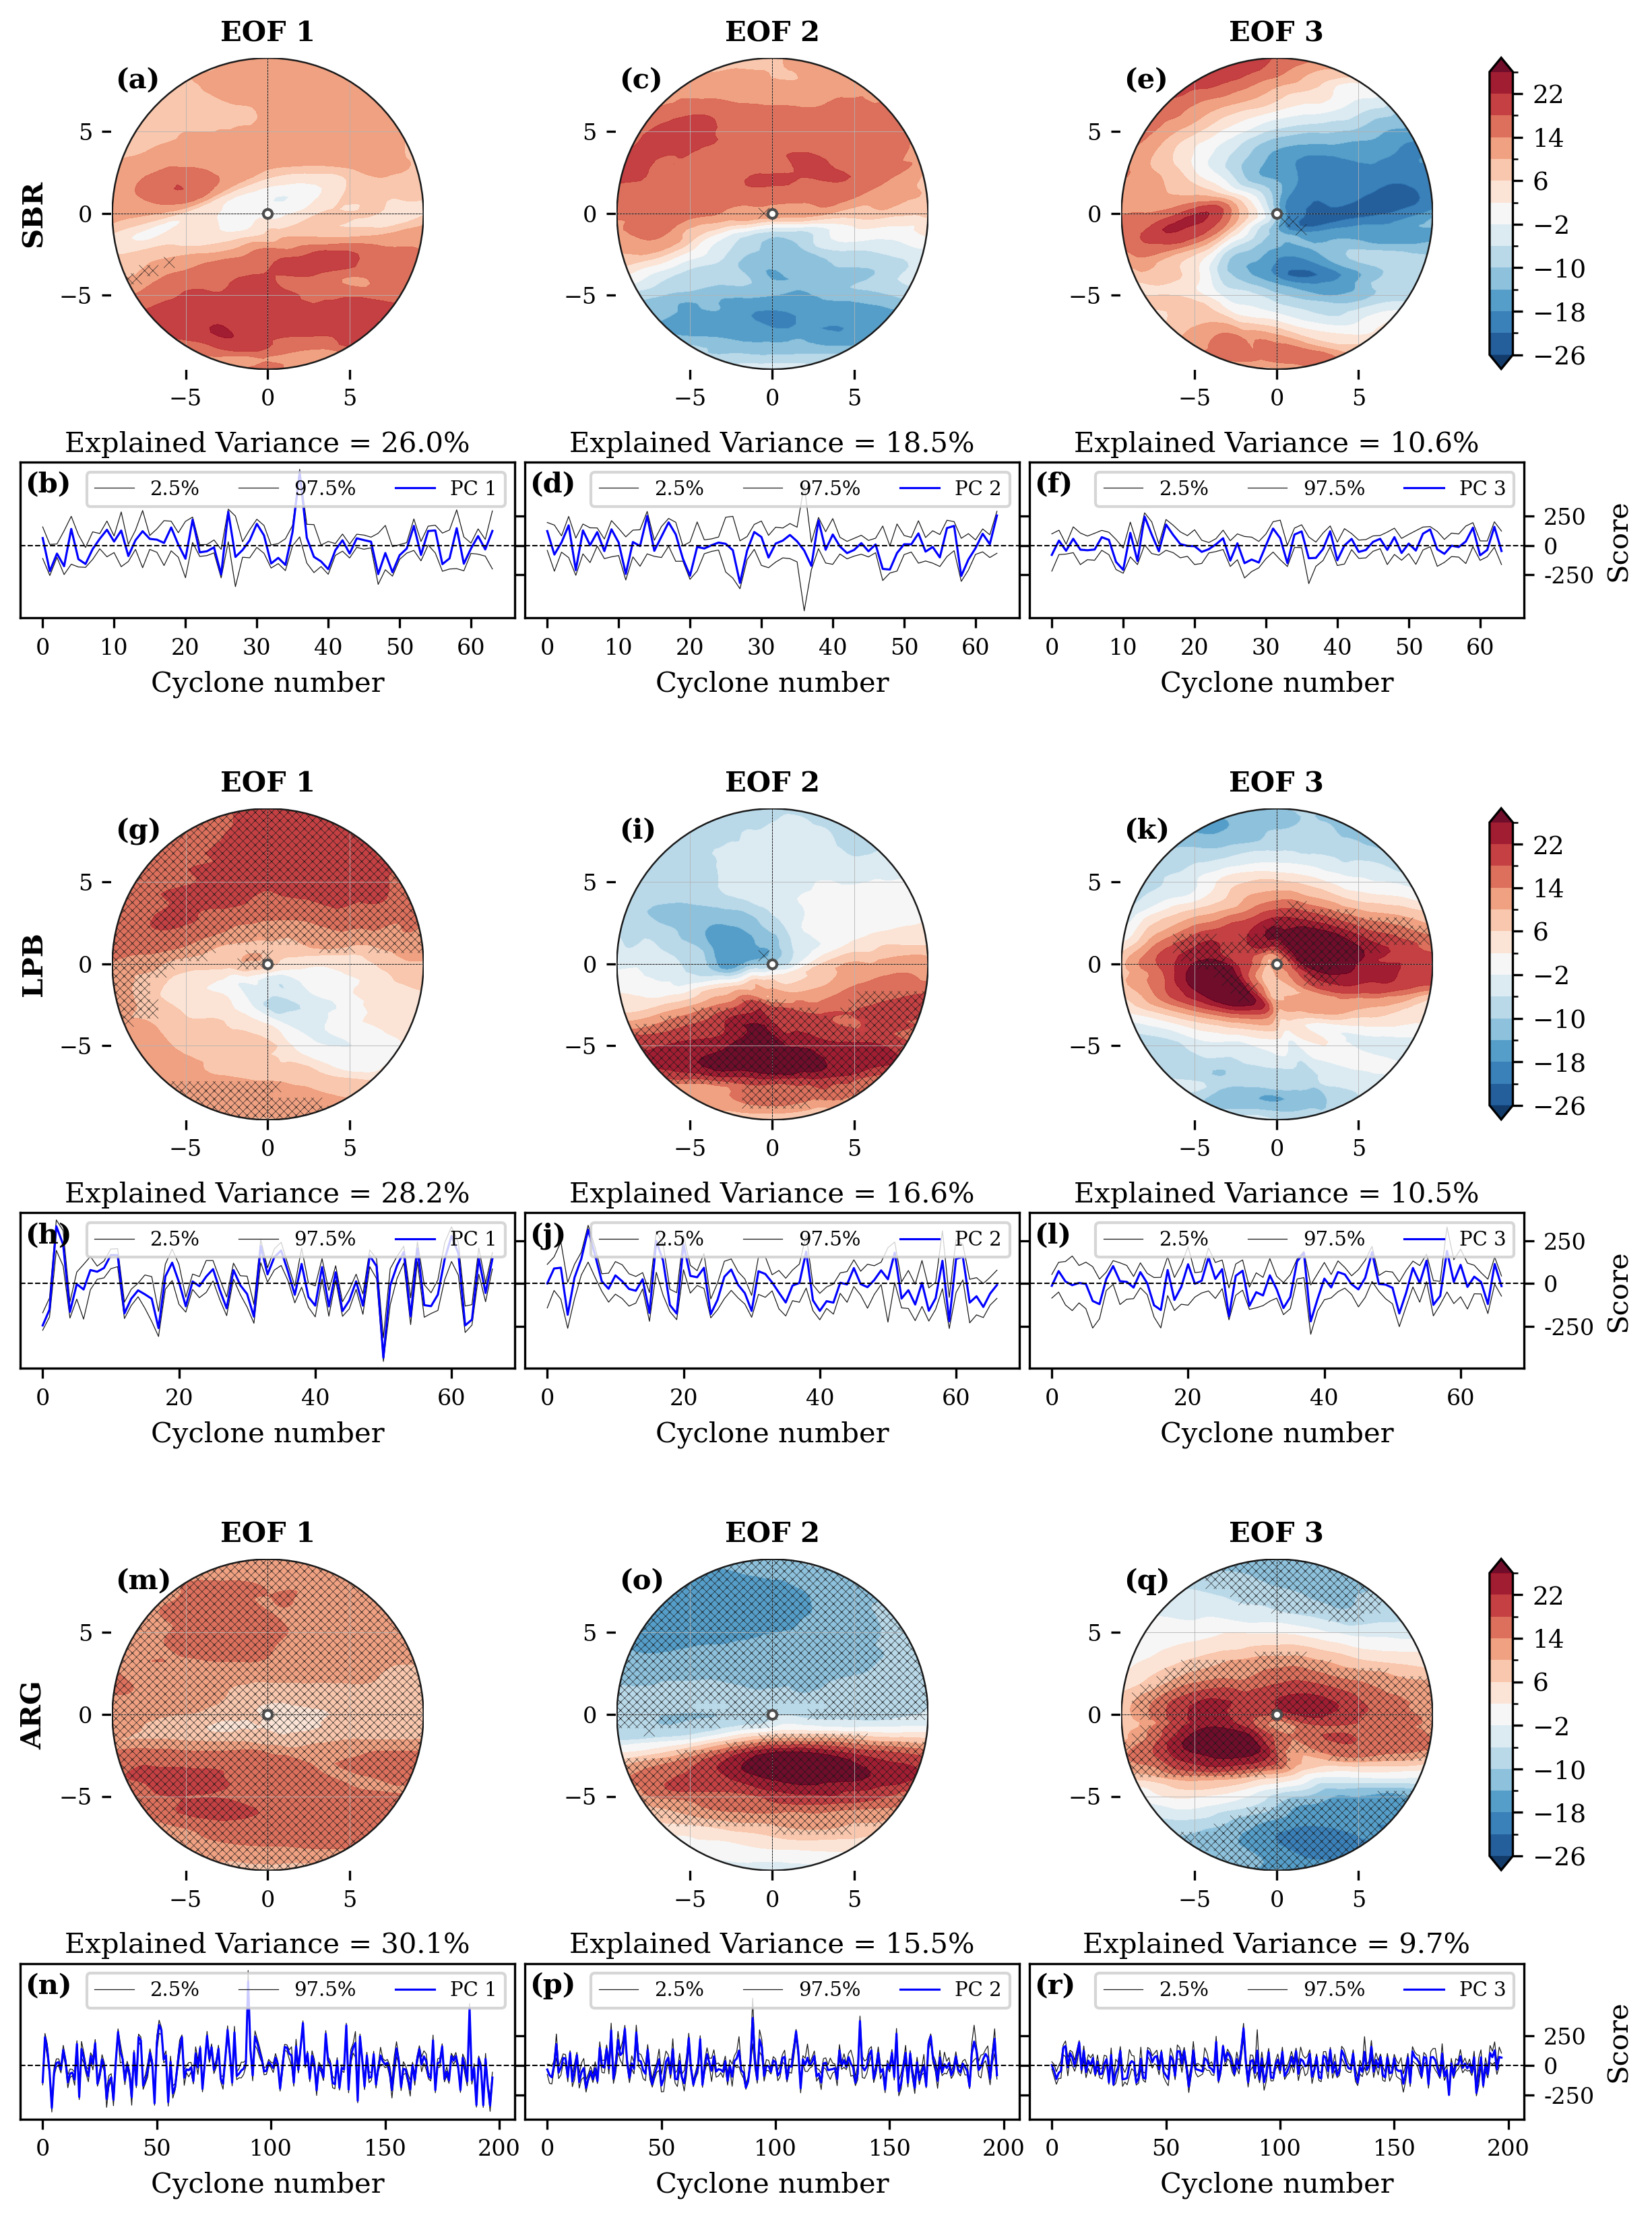
\includegraphics[width=\textwidth]{images/w10/xeof_p90_wind10_decay.jpg}
\caption[EOF1-3  - Subconjunto p90 (Decaimiento)]{Análisis multidimensional del viento a 10 metros para el \textbf{subconjunto extremo (p90)} durante la \textbf{fase de decaimiento}. Las zonas punteadas indican significancia estadística al 95\% empírico.}
\label{fig:apendice_p90_decaimiento}
\end{figure}
% ==============================================================================
% ==============================================================================
% ==============================================================================
\chapter{Análisis Multivariado Complementario (MEOF)}\label{apendice:meof}

% ==============================================================================
% FASE INCIPIENTE
% ==============================================================================
\section{Fase Incipiente: Viento a 100 metros y Precipitación (p10 y p50)}\label{apendice:meof_incipiente}

\begin{figure}[htbp]
\centering

\includegraphics[width=\textwidth]{images/meof/meof1_incipient_p10.png}
\caption[MEOF1 de viento a 100 m y precipitación (Incipiente) - p10]{Primer modo espacial multivariado (MEOF1) durante la fase incipiente para el estrato de baja intensidad dinámica (p10). La matriz organiza los resultados en columnas por región de ciclogénesis (SBR, LPB y ARG) y en filas emparejadas (la fila superior expone la anomalía de precipitación y la inferior su patrón covariante de viento a 100 metros). Con una varianza explicada de entre $12.7\%$ y $13.6\%$, la falta de covarianza espacial estructurada es casi absoluta, reflejando el ruido espacial de sistemas que carecen de un forzamiento inicial profundo.}
\label{fig:meof_incipiente_p10_ap}
\end{figure}

\begin{figure}[htbp]
\centering

\includegraphics[width=\textwidth]{images/meof/meof1_incipient_p50.png}
\caption[MEOF1 de viento a 100 m y precipitación (Incipiente) - p50]{Primer modo espacial multivariado (MEOF1) durante la fase incipiente para el estrato de intensidad moderada (p50). Manteniendo la misma disposición geométrica de filas emparejadas, este grupo (varianza entre $14.3\%$ y $19.1\%$) muestra los primeros indicios sutiles de alineación frontal entre ambas variables, sirviendo como la línea de base ideal para dimensionar la agresiva organización temprana que logran los eventos severos (p90).}
\label{fig:meof_incipiente_p50_ap}
\end{figure}

% ==============================================================================
% FASE DE INTENSIFICACIÓN
% ==============================================================================
\section{Fase de Intensificación: Viento a 100 metros y Precipitación (p10 y p50)}\label{apendice:meof_intensificacion}

\begin{figure}[htbp]
\centering

\includegraphics[width=\textwidth]{images/meof/meof1_intensification_p10.png}
\caption[MEOF1 de viento a 100 m y precipitación (Intensificación) - p10]{Primer modo espacial multivariado (MEOF1) durante la fase de Intensificación para el estrato p10. Al evaluar las filas emparejadas de precipitación y viento, se observa que el sistema retiene una covarianza sumamente difusa (varianza $\sim 13.8\%-15.1\%$), evidenciando su incapacidad termodinámica para organizar gradientes anómalos durante su etapa de profundización.}
\label{fig:meof_intensificacion_p10_ap}
\end{figure}

\begin{figure}[htbp]
\centering

\includegraphics[width=\textwidth]{images/meof/meof1_intensification_p50.png}
\caption[MEOF1 de viento a 100 m y precipitación (Intensificación) - p50]{Primer modo espacial multivariado (MEOF1) durante la fase de Intensificación para el estrato p50. Este grupo presenta una varianza conjunta del $11.5\%$ al $15.6\%$ y funciona como un escalón de transición estructural: las filas emparejadas comienzan a mostrar mayor superposición en sus señales, pero sin alcanzar jamás la violenta concentración asimétrica de los gradientes que distingue al estrato extremo (p90).}
\label{fig:meof_intensificacion_p50_ap}
\end{figure}

% ==============================================================================
% FASE DE MADUREZ
% ==============================================================================
\section{Fase de Madurez: Viento a 100 metros y Precipitación (p10 y p50)}\label{apendice:meof_madurez}

\begin{figure}[htbp]
\centering

\includegraphics[width=\textwidth]{images/meof/meof1_mature_p10.png}
\caption[MEOF1 de viento a 100 m y precipitación (Madurez) - p10]{Primer modo espacial multivariado (MEOF1) durante la fase de Madurez para el estrato p10, organizado en columnas (SBR, LPB, ARG) y filas emparejadas. Incluso en el momento de su máxima (aunque débil) vorticidad, el grupo mantiene un acople disperso y espacialmente ruidoso, capturando una varianza conjunta marginal (entre $14.3\%$ y $15.0\%$).}
\label{fig:meof_madurez_p10_ap}
\end{figure}

\begin{figure}[htbp]
\centering

\includegraphics[width=\textwidth]{images/meof/meof1_mature_p50.png}
\caption[MEOF1 de viento a 100 m y precipitación (Madurez) - p50]{Primer modo espacial multivariado (MEOF1) durante la fase de Madurez para el estrato p50. Con una varianza explicada del $10.7\%$ al $15.8\%$, el sistema logra delinear las bandas frontales básicas de lluvia y viento. Sin embargo, su superposición geográfica lineal es análoga al comportamiento de la Población Global, careciendo de la violenta expulsión periférica de humedad (desacople topológico) producida por el extremo forzamiento de los sistemas p90.}
\label{fig:meof_madurez_p50_ap}
\end{figure}

% ==============================================================================
% FASE DE DECAIMIENTO
% ==============================================================================
\section{Fase de Decaimiento: Viento a 100 metros y Precipitación (p10 y p50)}\label{apendice:meof_decaimiento}

\begin{figure}[htbp]
\centering

\includegraphics[width=\textwidth]{images/meof/meof1_decay_p10.png}
\caption[MEOF1 de viento a 100 m y precipitación (Decaimiento) - p10]{Primer modo espacial multivariado (MEOF1) durante la fase de Decaimiento para el estrato p10. Evaluado bajo el formato de matrices emparejadas, los mapas muestran la desorganización progresiva hacia el ruido ambiental tanto en el campo pluviométrico como cinemático, estabilizándose la varianza conjunta entre un $16.1\%$ y $17.6\%$.}
\label{fig:meof_decaimiento_p10_ap}
\end{figure}

\begin{figure}[htbp]
\centering

\includegraphics[width=\textwidth]{images/meof/meof1_decay_p50.png}
\caption[MEOF1 de viento a 100 m y precipitación (Decaimiento) - p50]{Primer modo espacial multivariado (MEOF1) durante la fase de Decaimiento para el estrato p50. Exhibe un patrón de disipación covariante suave (varianza entre $14.4\%$ y $19.1\%$), replicando la relajación homogénea y la pérdida conjunta de gradientes que caracteriza a los sistemas ordinarios al agotar su forzamiento dinámico y finalizar su ciclo de vida.}
\label{fig:meof_decaimiento_p50_ap}
\end{figure}


